% This is the Reed College LaTeX thesis template. Most of the work 
% for the document class was done by Sam Noble (SN), as well as this
% template. Later comments etc. by Ben Salzberg (BTS). Additional
% restructuring and APA support by Jess Youngberg (JY).
% Your comments and suggestions are more than welcome; please email
% them to cus@reed.edu
%
% See http://web.reed.edu/cis/help/latex.html for help. There are a 
% great bunch of help pages there, with notes on
% getting started, bibtex, etc. Go there and read it if you're not
% already familiar with LaTeX.
%
% Any line that starts with a percent symbol is a comment. 
% They won't show up in the document, and are useful for notes 
% to yourself and explaining commands. 
% Commenting also removes a line from the document; 
% very handy for troubleshooting problems. -BTS

% As far as I know, this follows the requirements laid out in 
% the 2002-2003 Senior Handbook. Ask a librarian to check the 
% document before binding. -SN

%%
%% Preamble
%%
% \documentclass{<something>} must begin each LaTeX document
\documentclass[12pt,twoside]{reedthesis}
% Packages are extensions to the basic LaTeX functions. Whatever you
% want to typeset, there is probably a package out there for it.
% Chemistry (chemtex), screenplays, you name it.
% Check out CTAN to see: http://www.ctan.org/
%%
%based off of cryptomacros file from Adam Groce for cryptography spring 2020
%this file is a mess since it is added packages and macros tacked on from outside sources :(

\usepackage{amsthm} %theorem environments etc
%\usepackage{fullpage} % reducing borders
%\usepackage{xspace}
\usepackage{amssymb} % \mathbb
\usepackage{amsmath}
\usepackage{amsfonts}
\usepackage[utf8]{inputenc}
%\usepackage{hyperref}
\usepackage{graphicx}
\usepackage[vlined]{algorithm2e}
\RestyleAlgo{boxruled}


\theoremstyle{remark}
\newtheorem*{rmk}{Remark}

\theoremstyle{plain}
\newtheorem{theorem}{Theorem}[chapter]
\newtheorem{corollary}[theorem]{Corollary}
\newtheorem{lemma}[theorem]{Lemma}
\newtheorem{prop}[theorem]{Proposition}

\theoremstyle{definition}
\newtheorem{dfn}[theorem]{Definition}

\setcounter{equation}{0}


\newcommand{\adv}{\mathcal{A}}
\newcommand{\reals}{\mathbb{R}}
\newcommand{\gen}{\ensuremath{{\sf Gen}}\xspace}
\newcommand{\enc}{\ensuremath{{\sf Enc}}\xspace}
\newcommand{\dec}{\ensuremath{{\sf Dec}}\xspace}
\newcommand{\negl}{\ensuremath{{\sf negl}}\xspace}
\newcommand{\EXP}{\mathbb{E}}
\newcommand{\bidders}{\textbf{b}}
\newcommand{\valuations}{\textbf{v}}
\newcommand{\strategies}{\textbf{s}}
\newcommand{\types}{\textbf{T}}
\newcommand{\actions}{\textbf{a}}
\newcommand{\OPT}{\text{OPT}}
\newcommand{\F}{\mathcal{F}}

\usepackage[procnames]{listings}
\usepackage{color}
\usepackage{xcolor}

\lstset{language=Python, 
	basicstyle=\ttfamily\small, 
	keywordstyle=\color{keywords},
	commentstyle=\color{comments},
	stringstyle=\color{red},
	showstringspaces=false,
	identifierstyle=\color{green},
	procnamekeys={def,class}}

%\usepackage{systeme}

%\usepackage[textheight=8.5in, margin=1.6in]{geometry}
\usepackage[total={6in,8in}]{geometry}

\usepackage{graphicx}

% Tikz stuff: This comes from Dave, hence it being added on at end
\usepackage{tikz}
\usetikzlibrary{shapes.misc, positioning}
\usepackage{pgfplots}
\pgfplotsset{compat=1.13}
%\usepgfplotslibrary{fillbetween}
%\usetikzlibrary{cd}
%\usetikzlibrary{graphs,graphs.standard}
%\usetikzlibrary{decorations.pathmorphing}    
%\usetikzlibrary{decorations.pathreplacing}
%\usetikzlibrary{arrows.meta,calc}
%\usetikzlibrary{bending}
\usetikzlibrary{decorations.markings,shapes.geometric}
\tikzset{->-/.style={decoration={markings, mark=at position #1 with
			{\arrow{>}}},postaction={decorate}}}
\tikzset{-|-/.style={decoration={markings, mark=at position #1 with
			{\arrow{stealth}}},postaction={decorate}}}
\tikzset{movearrow/.style 2 args ={
		decoration={markings,
			mark= at position {#1} with {\arrow{#2}} ,
		},
		postaction={decorate}
	}
}
\tikzset{<--/.style={decoration={markings, mark=at position #1 with
			{\arrow{<}}},postaction={decorate}}}
\tikzstyle{ball} = [circle,shading=ball, ball color=black,
minimum size=1mm,inner sep=1.3pt]
\tikzstyle{bball} = [circle,shading=ball, ball color=blue,
minimum size=1mm,inner sep=1.3pt]
\tikzstyle{miniball} = [circle,shading=ball, ball color=black,
minimum size=1mm,inner sep=0.5pt]
\tikzstyle{redminiball} = [circle,shading=ball, ball color=red,
minimum size=1mm,inner sep=0.5pt]
\tikzstyle{mminiball} = [circle,shading=ball, ball color=black,
minimum size=0.6mm,inner sep=0.1pt]
\tikzstyle{mycircle} = [draw,circle, minimum size=1mm,inner sep=1.3pt]

\usepackage{needspace}  % <-- to prevent bad pagebreak over environment titles
% Use:  \Needspace{3\baselineskip} before opening an environment

\usepackage{enumitem}
%\setlist[enumerate]{leftmargin=*}
\setlist[enumerate]{itemsep=2pt,label={(\alph*)}}

%\allowdisplaybreaks
%\usepackage[colorlinks=true,citecolor=black,linkcolor=black,urlcolor=blue]{hyperref}
%\usepackage{algorithm}
%\usepackage[noend]{algpseudocode}

\usepackage{outlines}



	
	



\usepackage{graphicx,latexsym} 
\usepackage{amssymb,amsthm,amsmath}
\usepackage{longtable,booktabs,setspace} 
\usepackage{chemarr} %% Useful for one reaction arrow, useless if you're not a chem major
\usepackage[hyphens]{url}
\urlstyle{same}
\usepackage{rotating}
\usepackage{natbib}
\usepackage{changepage}
\usepackage[vlined]{algorithm2e}
\usepackage{amsthm}
\usepackage [english]{babel}
\usepackage [autostyle, english = american]{csquotes}
\MakeOuterQuote{"}

\graphicspath{./diagrams/}
% Comment out the natbib line above and uncomment the following two lines to use the new 
% biblatex-chicago style, for Chicago A. Also make some changes at the end where the 
% bibliography is included. 
%\usepackage{biblatex-chicago}
%\bibliography{thesis}

% \usepackage{times} % other fonts are available like times, bookman, charter, palatino

\title{Simulating the Price of Anarchy in Auctions}
\author{Robert S. Irvin}
% The month and year that you submit your FINAL draft TO THE LIBRARY (May or December)
\date{May 2020}
\division{Economics and Mathematics}
\advisor{Jeffery Parker}
%If you have two advisors for some reason, you can use the following
\altadvisor{David Perkinson}
%%% Remember to use the correct department!
\department{Economics-Mathematics}
% if you're writing a thesis in an interdisciplinary major,
% uncomment the line below and change the text as appropriate.
% check the Senior Handbook if unsure.
\thedivisionof{The Established Interdisciplinary Committee for}
% if you want the approval page to say "Approved for the Committee",
% uncomment the next line
\approvedforthe{Committee for}

\setlength{\parskip}{0pt}
%%
%% End Preamble
%%
%% The fun begins:
\begin{document}

  \maketitle
  \frontmatter % this stuff will be roman-numbered
  \pagestyle{empty} % this removes page numbers from the frontmatter

% Acknowledgements (Acceptable American spelling) are optional
% So are Acknowledgments (proper English spelling)
    \chapter*{Acknowledgments}
	Thank you to all of my friends and family who helped me reach the end. Most especially I would like to thank Ryan Gamblin whose steadfast friendship has meant everything over these past years, and Jasmine Holland whose direct support on this thesis and getting through quarantine have made all of this possible. I would like to thank my parents who always encouraged me to stretch myself academically, even if that meant traveling so far away. I would like to thank my brother who patiently taught me how to code last summer, and who always answered my technical questions as they came up writing this thesis. Finally I would like to thank all of my friends, teachers, and professors who made contributions large and small to my education and my life. Without all of these people I could not be here, nor would I want to.

% The preface is optional
% To remove it, comment it out or delete it.
%    \chapter*{Preface}
%	"For if we could suppose a great multitude of men to consent in the observation of justice and other laws of nature without a common power to keep them in awe, we might as well suppose all mankind to do the same; and then there neither would be, nor need to be, any civil government or commonwealth at all, because there would be peace without subjection." -Thomas Hobbes (Leviathan, chapter XVII)
	
	%TODO find a better leviathan quote
	
	

%    \chapter*{List of Abbreviations}
%
%	\begin{table}[h]
%	\centering % You could remove this to move table to the left
%	\begin{tabular}{ll}
%		\textbf{AI}  	&  Artificial Intelligence\\
%		\textbf{MAS}  	&  Multi-Agent System\\
%		\textbf{ML}     &  Machine Learning\\
%		\textbf{POA}    &  Price of Anarchy
%	\end{tabular}
%	\end{table}
	

    \tableofcontents
% if you want a list of tables, optional
%    \listoftables
%% if you want a list of figures, also optional
%    \listoffigures

% The abstract is not required if you're writing a creative thesis (but aren't they all?)
% If your abstract is longer than a page, there may be a formatting issue.
    \chapter*{Abstract}
    
    The purpose of this thesis is to demonstrate via simulation the efficiency guarantees of the price of anarchy in first-price, single-item auctions. An agent based model is used where each agents strategy can be updated to demonstrate the efficiency properties of the system under this strategy. 
    
    The simulations find that agents using known Bayes-Nash equilibria strategies converge to a price of anarchy greater then the lower bound given by theory. Next, we see that agents who use an arbitrary bidding strategy still achieve high efficiency in both symmetric and asymmetric auctions despite their lack of intelligence, and that as the number of bidders increases these auctions approach full efficiency. Finally, we see that no-regret learning agents converge to outcomes both better than the efficiency guarantees that theory would suggest, and better than the arbitrary bidders.  
    
    The results from this experiment both demonstrate the correctness of the price of anarchy theory and give high confidence in efficiency of first-price single-item auctions. While even arbitrary agents perform quite well, we see that agents who are capable of learning and reflecting human behavior converge to highly efficient outcomes.  
	
%	\chapter*{Dedication}
%	You can have a dedication here if you wish.

  \mainmatter % here the regular arabic numbering starts
  \pagestyle{fancyplain} % turns page numbering back on

%The \introduction command is provided as a convenience.
%if you want special chapter formatting, you'll probably want to avoid using it altogether

    \chapter*{Introduction}
         \addcontentsline{toc}{chapter}{Introduction}
	\chaptermark{Introduction}
	\markboth{Introduction}{Introduction}
	% The three lines above are to make sure that the headers are right, that the intro gets included in the table of contents, and that it doesn't get numbered 1 so that chapter one is 1.

% Double spacing: if you want to double space, or one and a half 
% space, uncomment one of the following lines. You can go back to 
% single spacing with the \singlespacing command.
% \onehalfspacing
\doublespacing

When people act rationally, society can suffer. Economists often talk about the tragedy of the commons, a scenario where people follow their incentives to over-utilize a public good and ruin it for society at large. In the tragedy of the commons, each agent's rational behavior is what leads the system to converge to overuse, wasted resources, and utility lower in the long run than if they had been able to preserve the resource. While the idea of the tragedy of the commons is about how incentives can lead to the overuse of public resources, there is a larger problem at the heart of it: how and why is it that when people behave strategically it often leads to worse outcomes for both the individual and society as a whole? 

The fact that selfish behavior leads to a worse outcome in the tragedy of the commons is a product of the system it takes place in. Because the incentives of this game line up with individualistic choices that are bad for society, rational agents will always choose to over-utilize the public good. It would only be if some outside force came in and made people behave correctly that these agents could maintain behaviors that would lead to the best outcome for society in the long run. Socially optimal choice for all agents is not an equilibrium when agents behave rationally in this case, but we can still imagine what it would be like if agents were forced to make socially responsible choices by some external force. This is an economic dream, to have some {\em deus economica} control the actions of every agent to maximize some empirically derived social welfare function. Every action pre-planned and every util maximized for the good of us all. In lieu of an economic god ruling us, maybe some benevolent dictator could be set up instead? 

Even if a benevolent dictator can be found, who is to say that they will be able to calculate the exact optimal solutions for large scale problems? Imagine a nation's government trying to calculate the socially optimal number of shoes to manufacture each year for millions of people each with different shoe sizes and preferences? It seems doubtful that any government would be capable of doing this as there is too much data to process and too many changing circumstances to react quickly to societal need. Rather, most countries leave shoe manufacturing to a free market which has firms that can pop up and respond to the demands of customers at will. That is not to say that the free market is perfect for shoes: we have no way of knowing if its allocation of resources end up being the best possible. In fact, it is highly doubtful that it is. There is only one socially optimal outcome (which presumably our omnipotent god of economics could calculate) but there exist an infinite number of outcomes which are worse than optimal. Our question is one of trying to understand what makes some markets or systems behave in a way that is good for society and some terrible for society when everyone is behaving selfishly, or, how can we describe the effect of selfish behavior on a system. One way of approaching an answer to this question is instead of trying to understand how agents behave in the worst case (from a social welfare perspective) for a given system or game. That is, we want to bound the systems worst possible social cost when people are behaving rationally. This is called the {\em price of anarchy}, the worst possible price paid in terms of social welfare  at the equilibria for rational agents within that system. 

The idea of equilibria in a system is also problematic. How are we to presume that agents converge to an equilibria? Are they able to easily calculate it and decide to go there to begin with? No. We should be concerned with the set of outcomes or equilibria that happens not only for fully rational agents with infinite computational power, but also with agents who learn how to behave as they participate, who dynamically react to the changes in strategy by the other players. 

This thesis is about simulating the price to society for anarchic behavior within a system (game) who learn to play as they go. Computer scientists and economists have been proving the bounds of this price for various systems both at the fully rational equilibria, and at the equilibria that certain learning agents converge to. We create a simulation to demonstrate this bound in one of the most simple markets, a sealed bid first-price, single-item auction. This is an auction where everyone bids simultaneously, one-shot on a single item and the highest bidder gets the item. Thus, by constructing a simulation of an auction in this way, we can be more sure that when this auction format is used in real life that these auctions are producing outcomes that are at least as efficient as our lower bound, and we no longer have to worry about finding a benevolent dictator.
	 
	
\chapter{Auctions and Computational Economics}
	Within the last three decades, computational economics has been on the rise. This branch of economic research encompasses two major ideas. One is that the increasing power of computers can help solve and understand classical economic problems through increasingly more complex simulations and numerical analysis. The other, is that the mathematical methods developed in the field of theoretical computer science can be used to explore existing models in economic theory in terms of their algorithmic and computational complexity. We aim to take elements from both of these frameworks, simulation and computational theory, to better understand the efficiency of one shot (first-price, sealed-bid) auctions at equilibrium. 

\section{Auctions, Equilibria, and Anarchy}
It is perhaps obvious why economists would be interested in studying auctions. Auctions are one of the most basic market structures that have roots going back to at least the ancient Greeks and still exist today in places such as art auctions and Ebay \citep{Mochon2015}. In the past 15 years, economists have been joined by computer scientists who are increasingly interested in the strategic interactions of agents within this setting. Christos Papadimitriou said in a 2015 lecture at the Simons Institute that it was the advent of the internet, an artifact out of computer scientists control, that turned theoretical computer science into a "physical science." Now computer scientists had to "approach the internet with the same humility that economists approach the market..." He went on to say that "it also turned us[, computer science,] into a social science. It was obviously about people and incentives. Without understanding this, you cannot understand the internet"\citep{Papadimitriou2015}. It is within this framework that he says computer scientists first began to study auctions as they existed on the internet such as Ebay and Google's sponsored search auctions. Now, computer scientists are moving beyond the internet, taking the mathematical tools of their discipline and applying them as a lens to understand and explain the world. This thesis is looking at the field of algorithmic game theory: the study of the algorithms and complexity of strategic interactions. For economists, this can be thought of as a new toolbox for unpacking and understanding the models and structures that already dominate the field. For example, in the case of a Walrasian auctioneer who calculates the clearing prices of a combinatorial auction, their problem was shown to be NP-complete, a complexity class usually called "intractable" due to the time it takes to solve these problems: the best algorithms here are generally guess and check, which gets out of hand for large inputs.\footnote{NP is the class of problems that a given solution can be checked in polynomial time, i.e.~$O(n^k)$ operations where $n$ is the size of the input and $k$ is any positive integer. NP-complete means that all problems in NP reduce to solving this problem. This is when you may hear "taking more time to compute than the age of the universe" etc.} Calculating Nash equilibria was shown to be a PPAD-complete problem, a complexity class somewhere between polynomial time and non-polynomial time \cite{Papadimitriou2015}. Using this, economists can further question the assumptions they are making about rational agents. When we assume agents in our models are calculating the Nash equilibria, is it reasonable given the complexity class of this problem? If in its hardest case we are assuming our agents are solving {\em intractable problem}, ones that's computation time grows very quickly with the size of its inputs, we may want to reconsider how reasonable the model is.

\subsection{The Price of Anarchy}
One of the major ideas to come out of algorithmic game theory is the \textit{price of anarchy} (POA), a mathematical way of showing the difference between the social welfare in the optimal case and in the worst case equilibrium for a game. This term was first coined by two computer scientists Elias Koutsoupias and Christos Papadimitriou, who were using the price of anarchy to understand network games and more generally were looking at how this concept could be used to understand behavior on the internet \citep*{Koutsoupias1999, Papadimitriou2001}. More formally, the price of anarchy for a game is the ratio of the minimum equilibrium social welfare in a game over the best possible social welfare of the game (see Definition \ref{dfn:POA}) An illustrative example of the price of anarchy from \citet[15-16]{Roughgarden2016} are selfish routing games played on graphs such as the one pictured below in figure \ref{braess}.

\begin{figure}[h!]
	\begin{tikzpicture}[scale=3.0]
	\node[circle,draw,inner sep=3pt, minimum size=15pt] at (0,0) (left) {$s$};
	\node[circle,draw,inner sep=3pt, minimum size=15pt] at (1,1) (top) {};
	\node[circle,draw,inner sep=3pt, minimum size=15pt] at (1,-1) (bottom) {};
	\node[circle,draw,inner sep=3pt, minimum size=15pt] at (2,0) (right) {$t$};
	\draw[->] (left)--(top) node[midway,above,rotate=45] {$c(x)=x$};
	\draw[->] (top)--(right) node[midway,above,rotate=-45] {$c(x)=1$};
	\draw[->] (top)--(bottom) node[midway,above,rotate=-90] {$c(x)=0$};
	\draw[->] (left)--(bottom) node[midway,below,rotate=-45] {$c(x)=1$};
	\draw[->] (bottom)--(right) node[midway,below,rotate=45] {$c(x)=1$};
	\end{tikzpicture}
	\centering
	\caption{Routing game from s to t. Strategic interaction will make everyone worse off.}
	\label{braess}
\end{figure}

In this game, each player chooses which edges to take on the directed graph from the source $s$ to reach the terminal $t$. Each edge has an associated cost, $c(x)$, expressed as a function of the proportion of players who take that edge, $x$. Player's total cost is then the sum of the costs for each of the edges they took to reach $t$. Player's objective is to minimize their total cost of reaching the terminal by picking the best route they can. In the game depicted in \ref{braess}, we see that routes either cost, 0, 1, or $x$, where $x$ is the proportion of the players who take that route ($x \in [0,1] $) 
For example if $50 \%$ of the players take that edge then $x=0.5$. This can be seen as analogous to traffic when driving a car, the more people take a road, the slower the traffic goes and the longer it takes to get somewhere. Knowing this, each player try to choose which path to take to get to their destination as quickly as possible. As you can quickly verify, the best solution for society, minimizing the total driving time for all, is when half of the drivers take the top route, and half of the drivers take the bottom route costing in total 1.5 for each driver. 

\begin{figure}[h!]
	\centering
	\begin{tikzpicture}[scale=3.0]
	\node[circle,draw,inner sep=3pt, minimum size=15pt] at (0,0) (left) {$s$};
	\node[circle,draw,inner sep=3pt, minimum size=15pt] at (1,1) (top) {};
	\node[circle,draw,inner sep=3pt, minimum size=15pt] at (1,-1) (bottom) {};
	\node[circle,draw,inner sep=3pt, minimum size=15pt] at (2,0) (right) {$t$};
	\draw[->,red,thick] (left)--(top) node[midway,above,rotate=45] {$c(x)=x$};
	\draw[->,red,thick] (top)--(right) node[midway,above,rotate=-45] {$c(x)=1$};
	\draw[->] (top)--(bottom) node[midway,above,rotate=-90] {$c(x)=0$};
	\draw[->,cyan,thick] (left)--(bottom) node[midway,below,rotate=-45] {$c(x)=1$};
	\draw[->,cyan,thick] (bottom)--(right) node[midway,below,rotate=45] {$c(x)=1$};
	\end{tikzpicture}
	\caption{Socially optimal routing, not at equilibrium}
	\label{braess2}
\end{figure}

However, this is not an equilibrium. The drivers taking the top route have incentive to instead take the middle edge to try and lower their total time traveled. In fact, the Nash equilibrium will end with all of the drivers taking the top x, going through the middle, and then the bottom x. Only then will no players have reason to deviate. These actions to individually and strategically try to decrease their cost end up producing a worse outcome for all players and society as a whole (the social welfare).\footnote{A careful observer will note that if the edge with cost 0 were not there, this would not be a problem. This is called Braess's Paradox where having this extra edge counter intuitively leads to worse outcomes \citep{Braess1968}.}  

\begin{figure}[h!]
	\centering
	\begin{tikzpicture}[scale=3.0]
	\node[circle,draw,inner sep=3pt, minimum size=15pt] at (0,0) (left) {$s$};
	\node[circle,draw,inner sep=3pt, minimum size=15pt] at (1,1) (top) {};
	\node[circle,draw,inner sep=3pt, minimum size=15pt] at (1,-1) (bottom) {};
	\node[circle,draw,inner sep=3pt, minimum size=15pt] at (2,0) (right) {$t$};
	\draw[->,blue,thick] (left)--(top) node[midway,above,rotate=45] {$c(x)=x$};
	\draw[->] (top)--(right) node[midway,above,rotate=-45] {$c(x)=1$};
	\draw[->,blue,thick] (top)--(bottom) node[midway,above,rotate=-90] {$c(x)=0$};
	\draw[->] (left)--(bottom) node[midway,below,rotate=-45] {$c(x)=1$};
	\draw[->,blue,thick] (bottom)--(right) node[midway,below,rotate=45] {$c(x)=1$};
	\end{tikzpicture}
	\caption{Route under strategic interaction, the only Nash equilibrium}
	\label{braess3}
\end{figure}

Now, it will take time $2$ for each player to reach the terminal. Thus, under strategic interaction we see that the equilibrium is {\em sub-optimal} for society: this set of player choices does not maximize the social welfare (by not minimizing the social cost). Moreover, in this specific case all individual players will be worse off under the equilibrium outcome than under the socially optimal one! So, the ratio of the social cost (total costs to all players) for the worst possible equilibria compared to the best possible, socially optimal (but not necessarily equilibria) outcome can be computed $$\frac{\sum_{n=1}^{N} n \cdot 2}{\sum_{n=1}^N n \cdot 1.5} = \frac{4}{3}$$ where we sum the cost for our $N$ players in each of the two scenarios described above depicted in figure \ref{braess2}, and figure \ref{braess3} \citep{Roughgarden2017}.\footnote{This is a cost minimization game so POA = EQ-social-cost/OPT-social cost. Definition \ref{dfn:POA}, is for auctions, a payoff maximization game, so POA = EQ-social-welfare/OPT-social-welfare. In general it is important to check if higher numbers are a good thing in that context!} Since this is a cost minimization game, $POA \geq 1$, and the closer the number is to one, the closer the worst case Nash equilibrium is to optimal. For this network, there is only one Nash equilibrium for selfish routing games, however, price of anarchy bounds can be found for the class of game as a whole regardless of its individual construction. These bounds tell us how much worse then optimal we can expect a system at equilibrium to behave in the worst case. The price of anarchy bound for the entire format of selfish routing games with affine cost functions (i.e. $c(x) = ax+b$) is know to be $4/3$. This means that our example is as bad as the price of anarchy can get for any network we construct to play a routing game \citep{Roughgarden2007}. 

\subsection{Auctions}
Researchers in algorithmic game theory have recently been applying the lens of the price of anarchy to understand the efficiency of auctions. This pursuit should seem very familiar to economists who traditionally want to understand the efficiency of market structures. To understand how the price of anarchy framework is helpful for auctions, it is first worth understanding the basics of auction theory and how it is that inefficiencies could arise. 

An \textit{auction} is a market mechanism, operating under specific rules that determines to whom one or more items will be awarded and at what price. To do this, an auctioneer solicits a bid, or a sequence of bids from each of the players for the items being auctioned and then uses some fixed rule (or mechanism) to determine who is awarded the items and how much each bidder must pay. While we may traditionally think about ascending auctions for a single item, called an {\em English auction}, where the auctioneer keeps soliciting higher and higher bids until no one is willing to bid anymore, this is not the only kind of auction. There can be many different rules for determining who the winner is, or what price each of the bidders must pay (regardless of if they win or not) \citep{Mochon2015}.

We use the notation from \cite{Mochon2015} to express auctions as mathematical objects. An auction consists of a set of $n$ {\em bidders} who are trying to buy the object and a {\em seller} who is trying to sell the object.  For each bidder $i$ in an auction, their {\em  valuation} $v_i$ is how much they value the item. This is sometimes called a private valuation as this value is generally unknown by the other participants in the auction. The \textit{bid}, $b_i$, is the offer that bidder $i$ submits for an item. {\em Sincere bidding} is when $v_i = b_i$, {\em underbidding} is when $v_i > b_i$, and {\em overbidding} is when $v_i < b_i$. The highest bid made by any bidder is denoted $b^*$, and under the highest price mechanism, $b^*_i$ is also the winning bid (if multiple bids equal the winning bid, then some tie-breaking rule must be used).\footnote{We could in principle also have a second (or j-th) highest price mechanism meaning that the second (or j-th) highest bidder would win the item. Obviously, depending on how many bids players are allowed to submit this will change how they play the game.} The \textit{selling price}, $p^*$ is the final price that the bidder actually pays for the item (which, depending on the auction type, need not equal $b^*$). Before the auction begins, each bidder only knows their private valuation for the item, and the distribution from which they believe the other bidders will be sampling their valuations. During the auction, the auctioneer solicits a number of bids from each of the player depending on the format of the auction. In a sealed bid auction for example, each bidder secretly submits only one bid to the auctioneer. The way that bidders decide how they are going to bid is called a {\em strategy}. A strategy is a mapping from their private valuation $v_i$ to their bid $b_i$. After the auction, the bidder $i$ wins the item if their bid is higher than the bid placed by any other bidder, $b_i > \max_{i \neq k} \{b_k\}$. In a single item auction, the {\em income of the bidder} $i$ is equal to their value of the item: $$ \Gamma_i^* = v_i$$ and the {\em surplus of the bidder} $i$ is equal to the difference between income and price paid $$ \Pi_i^* = \Gamma_i^* - p^*.$$ If a bid placed by a bidder is less than the winning bid, they do not win anything and their income and surplus are both zero. The {\em seller's revenue} in a single unit auction is equal to the price paid by the winning bidder $$ \mathcal{R} = p^*.$$ 

There are multiple different pricing rules in an auction that determine who gets allocated the item. In a {\em first-price} auction the winning bidder pays the amount of their bid, which is the highest bid of the auction: $p^* = b^*$. This first-price pricing rule is sometimes referred to as {\em pay-what-you-bid}. In a {\em second-price} auction, the winning bidder pays an amount that is equal to the second highest bid for the awarded item \citep{Vickrey1961} \footnote{The second price, sealed bid auction is also known as a Vickrey auction after the economist who invented it.}. In sealed bid auctions with a first-price rule, people must bid lower than their valuation if they want to get any surplus. In sealed bid auctions using the first-price rule, the agents must reason about how much less than their true valuation to bid, i.e.~how to {\em shade} their bid. Because no rational bidder would bid their true valuation in a first-price sealed bid auction, this leads to strategic interaction between the agents deciding how to bid, as well as potential inefficiency, awarding the item to a bidder who does not value the item the most. This stands in contrast with a second price auction which encourages bidders to bid their true valuations (as they will gain positive profits if they win no matter the second highest bid). This pricing mechanism aligns the incentives for bidders, bidding truthfully, with an efficient allocation of items \citep{Mochon2015}. However, we are concerned with inefficiency in auctions, not optimal outcome. Thus, we will confine ourselves to first-price sealed bid auctions as this simple auction has interesting bidding dynamics which price of anarchy analysis can shine a light on. Moving forward we will refer to sealed bid first-price auctions simply as first-price auctions as is common in the literature. 

Before discussing the known bounds on the price of anarchy for first-price, auctions, it is worth going deeper how the bids might lead to a non-optimal outcome and what we mean by that. Due to only knowing their own valuation of the good, each bidder must act under uncertainty as to how much they should bid to beat out the unknown valuations of the other bidders. However, if they bid their exact private valuation then they will get a surplus of zero, and zero utility. In order for them to get some utility for the item they must be paying less then the exact amount they value the item. How much each bidder should bid less than their valuation, or {\em shade}, their bid is determined by how much they think that the other party values the item. To capture this interaction, auctions are represented as Bayesian games (see Definition \ref{dfn:BayesianGame}) where each bidder is drawing their valuation from some a priori distribution. If one player knows that the other is drawing from a distribution with a smaller mean than they are (i.e.~probably doesn't value the item as much), the Bayes-Nash equilibrium (see \ref{dfn:BayesNashEQ}) will be at a point in the strategy space where the expected higher valuation bidder shades their less than the expected lower valuation bidder. In each of them doing so, they can maximize their expected payoffs based off of their beliefs for how the other player will bid. Importantly, this difference in shading can lead to the person who values the item most not winning the auction if they shaded their bid to much. Hence the {\em social welfare} (see Definition \ref{dfn:SocialWelfare}), the summed surplus of all bidders and the seller will be less than optimal at the Bayes-Nash equilibrium. 

The price of anarchy analysis for this format of auction has already been done, but the proofs are not complete. \cite{Syrgkanis2013} proved that the lower bound of the price of anarchy in first-price, single-item auctions is at least $1 - \frac{1}{e} \approx 0.63$. The exact upper bound is unknown, but it has been proven that it can be no better than $0.87$ \citep{Hartline2015}. This bound is true regardless of how many bidders there are or what distributions they are drawing their bids from. So, for any first-price single-item auction at equilibrium, we can say that the social welfare for any equilibrium must be at least $63\%$ of the optimal social welfare (the maximum possible social welfare achievable in this system). 

This moves us closer to understanding the social welfare produced by first-price single-item auctions, but these results do not pay attention to how the players arrive at these equilibria. Not to mention that in real world applications, we expect that players might play repeatedly in the same auction and learn as they play rather than come in with pre-computed strategies. This is especially true for when computing the equilibrium is computationally hard and the stakes of each individual auction is small. Given these observations, it is natural to ask questions about how the efficiency results carry over to adaptive game environments. One notion of learning  commonly used in both theoretical computer science and game theory is {\em no-regret learning}. An algorithm for a player satisfies the no-regret condition if, in the limit as the number of times the game is played goes to infinity, the average reward of the algorithm is at least as good as the average reward for the best fixed action in hindsight (assuming the sequence of actions for the other players remains unchanged) \footnote{That is to say that the algorithm will converge to having an average utility no worse than any fixed strategy we would have rather picked in hindsight after seeing the outcome for each of their actions (see Definition \ref{dfn:noregret}).}. The no-regret condition is not in itself a technique for learning, but rather a characteristic of a learning algorithm in a fixed action environment. It says that each player using an algorithm shown to satisfy the no-regret condition will do at least on average as well as if they had picked the best possible fixed action. If each player  incorporates this kind of learning algorithm, then it has been shown that these can converge to a larger class of equilibrium called {\em coarse-correlated equilibrium} where each player conditions their response on the expected action of the other player \citep{Blum2007}. Remarkably, \cite{Roughgarden2017}  produced a way to extend the price of anarchy bounds proven for Bayes-Nash equilibria to the larger set of coarse-correlated equilibria. Hence, that we know that the price of anarchy for the set of coarse-correlated equilibria for first-price, single-item auctions are also at least 0.63, and that if the bidders in the auction are no-regret learners, they can arrive at this equilibrium through the course of play.

We now state our goal: to simulate no-regret learning algorithms for agents in a first-price auctions for a single to demonstrate the price of anarchy for this auction format. Because algorithms exist that guarantee convergence to some equilibrium set, we can construct computer agents to carry out simulated auctions. Each agent will use the strategies dictated by the no-regret learning algorithm and because of the work on this literature, we know that we will see them converge to a coarse correlated equilibrium and we know that the efficiency of this learned equilibria must be at least 63\% of the optimal social welfare.

	
\section{Simulated Agents and Simulated Economies}
The history of computers in economics, as outlined in \citet{Backhouse2016}, goes all the way back to general purpose computers invented in the 1940's. At that time, Wassily Leontif used a computer to invert a 39 x 39 matrix to help solve his input output model. Since then, computers use in economics has exploded. With computers, economists are able to invert bigger matrices, do Monte-Carlo simulations, create multinomial probit models, use full information maximum likelihood estimation, and all of the other computationally intensive techniques that economists now take for granted. While we might say that one branch of computational economics is focused on creating stronger and stronger calculators to facilitate empirical research, another branch has focused on creating simulated economies that allow economists to construct a blended version of theory and research within a computer program. Within these simulated economies, theories can be coded into the simulation which, when run, can allow the researcher to conduct experiments that might not be practical to conduct in the real world. 

One kind of a simulation that can be run is called an agent-based model, a simulated system of autonomous decision makers (agents). These models are able to generate complex behavior even if only simple assumptions are made about the behavior of the coded agents. That is, these agents interacting with each other in complex ways are able to produce emergent phenomena in the macro structure of the system.

For example, in the late 1960's and early 1970's, Thomas Schilling created computer simulations to try to understand how and why self segregated neighborhoods formed. He coded a virtual environment where agents were given a simple preference, they are only happy if they are not the minority in their neighborhood and will keep moving otherwise \citep{Schelling1969}. This simple model can illustrate the main tenets of agent based modeling. We review a simplified implementation of this model outlined in Thomas Sargent and John Stachurski's 2019 lectures in quantitative economics.\footnote{These lectures are a treasure trove of information on how to use Python to construct economic models. The simulation in chapter three was built in part using them as a guide.} First, we have agents who are simple enough to be representative of people in the real world: they are only "happy" if half of their closest neighbors are the same as them. If they are not happy then they will move somewhere else arbitrarily. These preferences can be given as the short procedure, or algorithm, shown below where $L$ is just the space they live in:

\begin{adjustwidth}{1cm}{}
	\textbf{1.} draw a random location in $L$, \\
	\textbf{2.} if happy at new location, move there,\\
	\textbf{3.} else, go to step 1.
\end{adjustwidth}

In this case, we get to choose what that environment looks like and like Shelling we can just say that it is a one by one unit square and we can say that their neighbors are the ten closest people to them (in Euclidean distance) on that square. We ran this simulation (after constructing it in Python) with green and orange dots representing the types of people. There are 250 agents (125 green and 125 orange) in our simulation, and we conducted five cycles of the above procedure going through each of our 250 agents until everyone was "happy" and stopped moving.

\begin{figure}[h!]
	\centering
	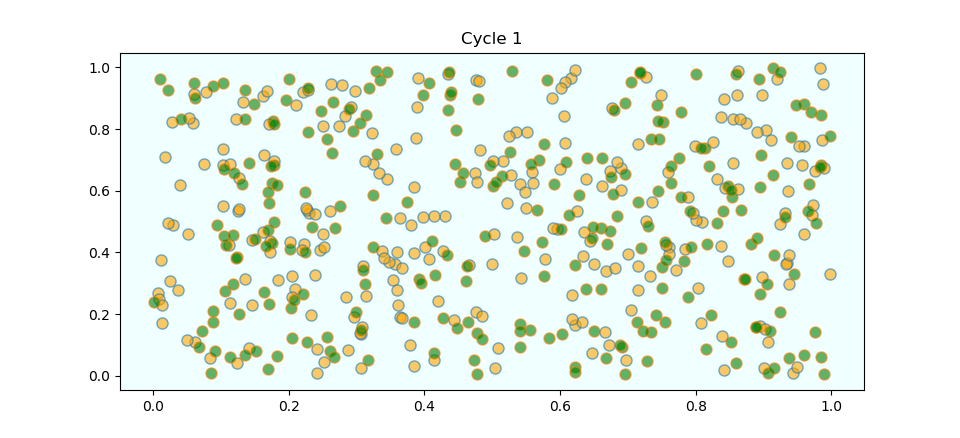
\includegraphics[scale=0.5]{Figures/segregation_1}
	\caption{Schelling's Segregation Model: Cycle 1}
	\label{SSM1_ch1}
\end{figure}

\begin{figure}[h!]
	\centering
	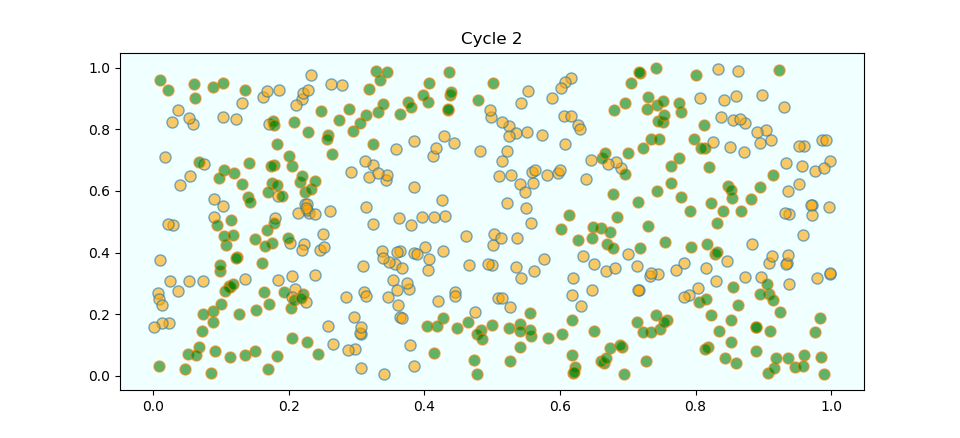
\includegraphics[scale=0.5]{Figures/segregation_2}
	\caption{Schelling's Segregation Model: Cycle 2}
	\label{SSM2_ch1}
\end{figure}
\begin{figure}[h!]
	\centering
	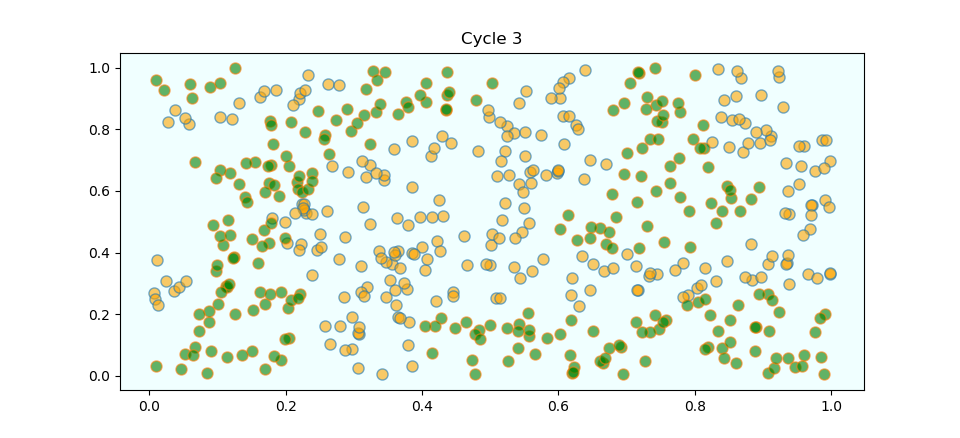
\includegraphics[scale=0.5]{Figures/segregation_3}
	\caption{Schelling's Segregation Model: Cycle 3}
	\label{SSM3_ch1}
\end{figure}
\begin{figure}[h!]
	\centering
	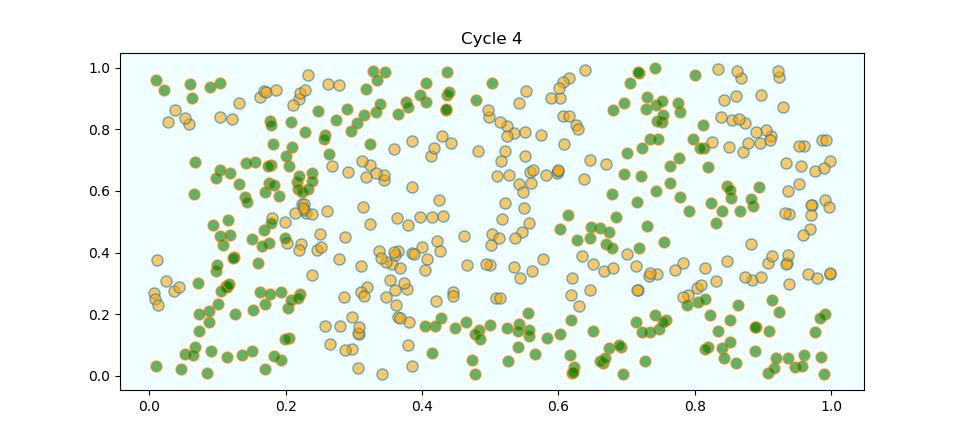
\includegraphics[scale=0.5]{Figures/segregation_4}
	\caption{Schelling's Segregation Model: Cycle 4}
	\label{SSM4_ch1}
\end{figure}
\begin{figure}[h!]
	\centering
	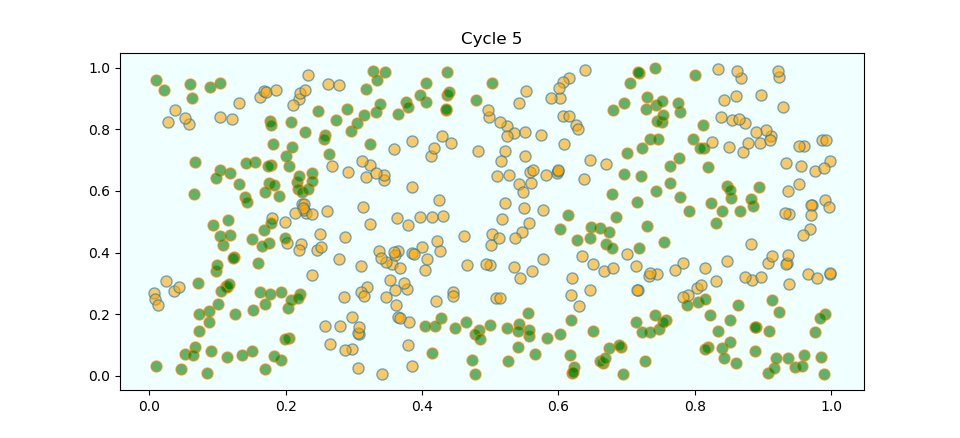
\includegraphics[scale=0.5]{Figures/segregation_5}
	\caption{Schelling's Segregation Model: Cycle 5}
	\label{SSM5}
\end{figure}

As can be seen, in cycle 1 (Figure \ref{SSM1_ch1}), the agents are well distributed among each other, but as they move in cycles 2-5, they become progressively more segregated. After 5 cycles all agents are happy and the simulation terminates. With very few assumptions about the agents' preferences, we can see the resulting emergent behavior of segregated neighborhoods in the system as a whole. Not only that, but the agents naturally move to an equilibrium as they adjust their behavior to what their neighbors are doing \citep{Sargent2019}. 

Agent based modeling has been used to build and understand much more complicated systems then the example illustrated above. The Santa Fe Institute in New Mexico is one of the main proponents of agent based modeling releasing a manifesto supporting the use of this technique to understand the {\em complexity} of economics from the ground up \citep{Backhouse2016}. They built the Santa Fe Artificial Stock Market in the 1990's to try and simulate the behavior of agents on the stock market and how using adaptive trading strategies effects the outcome of the market. The Santa Fe Artificial Stock Market is one of the first examples of agents learning and adapting to their environments as part of the simulation, and represents a move to model not only peoples preferences in simulations, but also how they learn and adapt\citep{LeBaron2002}. In the Santa Fe Artificial Stock Market, agents used a genetic algorithm to adapt their trading strategy at each period by modifying a string (for example $00011100$) where each bit in the string told the agent to use a certain behavior or not. Those trading strategies that did well were coded to survive longer where the agents with worse strategies would randomly modify their own or take a more successful agent's strategy \cite{Joshi1998}. This genetic algorithm was supposed to be representative of the learning of traders on the stock market so that the insights taken from running these agents in simulation could be applied to learn something about the real world \citep{Arthur1992}. 

The authors of Santa Fe Stock Market paper suggested that their genetic algorithm was one of many algorithms that could be used to stand in for human behavior saying that reinforcement learning or deep learning could also be used to stand in for human intelligence in a simulation\footnote{Reinforcement learning is when an algorithm plays a game repeatedly and updates its beliefs about what actions will lead to the best payoff. Deep learning uses deep neural networks to try and estimate the best outcomes in a fashion similar to regression.}. More specifically they suggest that an appropriate algorithms can be chosen so long as they behave reasonably well like humans in that scenario, something like a Turing test \citep{Arthur1991}.  Unfortunately, research that has compared the behavior of human agents in strategic settings to that of these algorithms have not found some general algorithm that best approximates human learning. From game to game, different algorithms more appropriately behave like humans who were experimentally playing the same games \citep{Tesfatsion2002}. Having no algorithm to approximate humans in a simulation is a problem only assuming that you want your agents to in some way represent human behavior; we might simply want our agents to represent the "rational choice" in any given situation. Unfortunately, the learning algorithms we have today aren't necessarily fully rational in the normal economics sense either. While the artificial agents may learn how to maximize their utility, in general learning algorithms are simply searching the space as best they can rather than computing outright how they should behave. As Holland and Miller say in their 1991 paper "Artificial Adaptive Agents in Economic Theory", "Usually there is only one way to be fully rational, but there are many ways to be less rational" (pg 367). Since they recognize the agents they are creating for their simulation probably fall in the "less rational" camp, they suggest to get around this is to try and build models that have robust behavior across agent learning algorithm choice. If most learning algorithms lead to similar results (for whatever you are trying to prove), we may be fairly confident that we are looking at a property of learning in the system that leads to the result you think you have demonstrated rather than the particular outcome reached by the specific algorithm you choose.

%(\cite{Rejeb2005}, \cite{Shoham2008})
%TODO Fix pg cite above

The literature of game theory provides another solution for trying to approximate human learning, no-regret learning. This is a simple learning requirement that means that this kind of algorithm should (hopefully) be more robust across representing human behavior. It also allows us to combine our simulated models and analytical models in a nice way. Because of the well described properties of no-regret algorithms, one can describe and prove the behavior of systems using this behavior in a stronger way than we ever could using a simulation. Since there are proven no-regret algorithms, we can also code this behavior into our simulated agents that might help us understand the system better than just looking at the analytical results.

Moving forward, this thesis aims to better understand the efficiency of auctions by simulating them using no-regret learning agents. The main aim of this simulation will be to demonstrate the price of anarchy bounds proven by \cite{Roughgarden2017}, and then to beyond that see how efficient we might expect these auctions to be not just in the worst case. We will do this with first-price, sealed-bid auction as they are the best understood theoretically and simple to code.

\chapter{Price of Anarchy in First-Price Auctions}
This chapter lays out the mathematical framework for modeling auctions as Bayesian games of incomplete information, formally defines the price of anarchy in auctions, and shows the bounds on the price of anarchy for sealed bid first-price, single-item auctions (which we will simply refer to as first-price auctions). It then follows up on this framework of analysis to show how these bounds can be extended to agents competing in auctions using learning algorithms with a property called "no-regret" learning. This chapter primarily follows from the work of Tim Roughgarden, Vasilis Syrgkanis, and \'Eva Tardos who not only are all individually active in the field of algorithmic game theory and auctions, but also jointly authored the 2017 paper "The Price of Anarchy in Auctions" that is a survey of the entire topic. This chapter will be giving the important theorems and ideas that primarily come from this work and the individual work of these three authors, explaining them, demonstrating proofs where appropriate, and reconstructing the important ideas that we will be using in our simulation.   

\section{Auctions as Bayesian Games}
Auctions are typically modeled as Bayesian games, also known as games with incomplete information. As you would expect, this is simply a type of game where the players don't know everything. While it is obvious why an auction consisting of the strategic interaction of bidders could be modeled as a game, how it should be modeled requires some thought. After all, while each bidder knows their own valuation of the item being sold, unless for some reason (and against their own interest) the other players announced their valuation of the item before the auction began our bidder will not know how the other players value the item. In fact, it is precisely this lack of information in sealed-bid auctions that makes them interesting! If all players came into an auction knowing the valuation of other players, for first-price, single-item auctions assuming there was no tie, the bidder with the highest value would always win by bidding the valuation of the next highest bidder. Rather it is the uncertainty that players face about the valuation of other players that make things interesting as players must guess how much they should shade their bid (as again no rational player will ever bid at or above their valuation) based off of what they know about other players. 

What can we say that bidders know about the valuations of other bidders? Certainly they do not know nothing as we all have reasonable expectations about what some item is worth to others. No one will value a candy bar at a million dollars. But a collector of candy bars might value it at a higher value than an ordinary person who just wants to eat the candy bar. For each bidder, we could can model them as drawing their valuation from some known distribution. As an example we might expect normal people's valuations of candy bars to be a normal distribution centered at \$1, but the collector's value might be a Laplacian distribution (allowing for more black swan events) centered at \$5. This sort of strategic interaction where the players know the distributions which parameters of the game are drawn from are typically called {\em games of incomplete information}, or {\em Bayesian games}.
 
\subsection{Bayesian Games}
Bayesian games of incomplete information are games in which one or more of the players lack "full knowledge" of the game that is being played. Introduced by John C. Harsanyi in 1967, rather than players knowing every parameter of the game situation such as utility functions, possible strategies, and information held by other players, each player knows a probability distribution from which these will be drawn. In his paper, Harsanyi says that this type of game can be thought of as a normal game, where "nature" goes first drawing from these probability distributions and assigning values before play begins without the players knowing which specific variation of the game they are playing \citep{Harsanyi1967}.
%TODO add page numbers when using quotes
 Importantly, each player does know the probability distributions from which each value is selected. Formally, slightly modifying the definition given in \citet{Nisan2007}, Bayesian games are defined as follows,

\begin{dfn}[Bayesian Game]
	A game with (independent private values and) \textit{incomplete information} on a set of $n$ players consists of:
	\begin{enumerate}
		\item For each player $i$, a set of {\em strategies} $S_i$, letting $S = S_1 \times \ldots \times S_n$.
		\item For every player $i$, a set of {\em types $T_i$}, and a prior distribution $F_i$ on $T_i$. A value $t_i \in T_i$ is the private information that $i$ has, and $\F_i(t_i)$ is the a priori probability that $i$ gets type $t_i$. $T = T_1 \times \ldots \times T_n$ and $\mathcal{F} = \mathcal{F}_1 \times \ldots \times \mathcal{F}_n$.
		\item For every player $i$, a \textit{utility function} $u_i : T_i \times S \rightarrow \mathbb{R}$, where $u_i(t_i, s_1, \ldots s_n)$ is the utility achieved by player $i$, if their type is $t_i$, and the profile of strategies played by all players is $s_1, \ldots s_n$.
	\end{enumerate} 
\label{dfn:BayesianGame}
\end{dfn}

We break down this definition before we apply it to auctions. For each player $i$, there is some set of strategies, or actions that they can take in the game, $S_i$. These strategy sets need not be finite, and they need not be the same for each player. In rock paper scissors of example $S_i = \{rock, paper, scissors\}$ for the two players $i =1$ and $i = 2$. Now, we create a larger set $S$, the {\em strategy space}, that is the Cartesian product of each individual players strategy sets. Elements of this set will then be the different possible strategy combinations. So, in the rock paper scissors example we get $S = \{rock, paper, scissors\} \times \{rock, paper, scissors\}$, and we can sample $\strategies \in S$ such as $\strategies = (rock, paper)$ or $\strategies = (rock, rock)$. We call these vectors $\strategies$, {\em strategy profiles}, where $\strategies = (s_1, \ldots, s_n)$. Often time, game theorists want to understand how a player $i$ would choose their strategy based off of the strategy of others. Hence, as is common in the literature, we let $\strategies_{-i}$ denote a strategy profile with the $ith$ element removed, the ordered vector of everyone else but player $i$'s strategies. In rock paper scissors if $s_{-i} = {rock}$, player $i$ would probably want to play paper, $s_i = paper$. 

The second part of Definition \ref{dfn:BayesianGame}, is what separates Bayesian games from normal mathematical games. We have a set of types for each player and some probability distribution over this set that tells how likely each player is to be of a certain type. We say that the probability distribution is {\em a priori} on the set of types which means that the probability of each type is known to the other players before the game starts. Here an illustrative example is are card games such as poker or five card draw. The type of each player would be their current hand of cards that they drew from the deck. Players only know their own cards, not the other players. They do however {\em a~priori} know how likely each possible hand is for the other player. In a card game, the probability distribution for types are not independent. If one player draws the ace of spades, the probability that the other player has a hand containing that card is zero (supposing they are using only one deck). To simplify talking about this, we will generally speak about drawing some type $t$ from $\mathcal{F}$.

The third part of Definition \ref{dfn:BayesianGame} is the utility function, $u_i$ for each player. This is a function that maps the strategies played by each of the players (which gives the outcome of the game), and the type of player they are to a real number, their "utility" for this outcome. We will often write $u_i(t_i, \strategies)$ instead of $u_i(t_i, s_1, \ldots s_n)$ for convenience. Players utility function, $u_i$, can be defined deterministically or probabilistically, for example as is common in the case that both players play strategies that leads to a tie, say $\strategies = (rock, rock)$ for rock-paper-scissors, one might let the tie be broken arbitrarily and have the winning player get the utility.


\subsection{First-Price Auctions}
We now move to using the formal structure of Bayesian games to model auctions. Here the types of players will be their valuation, $v_i$. As discussed in chapter one, $v_i$ represents how much bidder $i$ values the item being bidded on. There is also $\mathcal{F}_i$, the publicly known distribution over the set of valuations from which bidders are drawing their valuation for the item being auctioned. For example if each of the players was uniformly drawing their valuation from $[0,1]$, then their type $t_i$, would be $t_i \in T_i = \{x | 0 \leq x \leq 1\}$ and $\mathcal{F}_i$ is the uniform distribution over $T_i$. To avoid confusion in the notation, we will generally just speak of players drawing their valuation $v_i$ from their distribution $\mathcal{F}_i$ which we will write as $v_i ~ F_i$, and avoid talking about the type of the bidder. So, in Bayesian auctions bidders know their own valuation of the item being bidded on and the distribution from which each of the other players are drawing their valuations. In a sealed-bid first-price, single item auction if player $i$ wins with bid $b_i$, we define the utility of the winner to be $u_i = v_i - b_i$, the difference between their valuation and their bid and the losers all get $u_i = 0$ since they did not receive the item. Using the language of auctions, we are saying they are receiving utility equal to their surplus. A strategy for a player is a function $s_i \in S_i$ that maps a valuation $v_i$ in support of $\F$ to a bid, $b_i = s_i(v_i)$ (i.e.~taking into account the non-zero parts of the probability distribution for the other bidders valuations). 

We now move on to the idea of equilibrium in this system. In games of complete information the central equilibrium concept is usually a Nash equilibrium, the set of strategies for all players in which each individual player cannot increase their utility by deviating from their strategy fixing the strategy of all the other players. That is, for every player if no one else changes strategy, their best option is to stay where they are, hence an equilibrium. This concept is now updated to give us a Bayes-Nash equilibrium where we must also incorporate the distributions which players are drawing from. For an auction, Bayesian-Nash equilibria are defined as follows by \cite{Roughgarden2017}:

\begin{dfn}[Bayes Nash Equilibrium Auctions]
	A strategy profile $\textbf{s}$ constitutes a {\em Bayes-Nash equilibrium} if for every player $i$ and every valuation $v_i$ that the player might have, the player chooses a bid $s_i(v_i)$ that maximizes her conditional expected utility where the expectation is over the valuations of the other players, conditioned on a bidder $i$'s valuation being $v_i$.
	\label{dfn:BayesNashEQ} 
\end{dfn}

This is an equilibria because, for the given strategy profile $\textbf{s}$, every player $i$ is maximizing their expected utility with their current choice of $s_i$. Hence, no player has incentive to deviate from their chosen strategy with this profile.
 
 Now, if for a bid profile $\textbf{b} = (b_1, \ldots, b_n)$, we let 
\[
	x_i(\textbf{b}) =
	\begin{cases}
		1 & \text{if player $i$ is the winner} \\
		0 & \text{otherwise},
	\end{cases}
\]

then the utility a player $i$ receives when their valuation is $v_i$ is 
$$u_i(\textbf{b}; v_i) = (v_i - b_i) \cdot x_i(\textbf{b}),$$ and we can say that a strategy profile $\strategies = (s_1, \ldots, s_n)$ is a Bayes-Nash equilibrium if and only if


$$ \EXP_{\textbf{v}_{-i} \sim \mathcal{F}_{-i}} [u_i(\textbf{s} (\textbf{v}); v_i) \ | \ v_i] \geq \EXP_{\valuations_{-i} \sim \mathcal{F}_{-i}} [u_i(b^{'}_i, \strategies_{-i}(\valuations_{-i}); v_i) \ | \ v_i] $$ where the expectation is over the prior distribution $\mathcal{F}$ \citep{Roughgarden2017}. So, the above equation is one way of symbolically writing Definition \ref{dfn:BayesianGame} for auctions.

\subsection{Example Auction}
We now turn to an example auction to clarify what has just been laid out. In this example we analyze an auction between two players, Alice and Bob, who are bidding on a candy bar where each draw their valuations from the uniform distribution on $[0,1]$. This is a first-price, sealed-bid auction where they each submit a bid for a (single) candy bar simultaneously. How are Alice and Bob supposed to decide what to bid on this auction? Supposing that Alice and Bob can calculate a Bayes-Nash equilibrium for this example, and that example is unique, they would know that their best strategy would be to bid their strategy at this equilibrium. But how would our bidders go about calculating the equilibrium? We recreate the proof of the existence of such an equilibrium as from \cite{Nisan2007}. An example of proving the uniqueness of this equilibria appears in \cite{Levin2002}.

\begin{prop}
	In a first-price auction among two players with prior distributions distributions of their valuations $v_1,v_2$, uniform over the interval $[0,1]$ the unique Bayesian-Nash equilibrium is $\strategies = (s_1(v_1) = v_1 / 2, s_2(v_2) = v_2 / 2)$.
\end{prop}

\begin{proof}{\citep{Nisan2007}}
	First we show that this is a Bayesian-Nash equilibrium. Let us consider which bid $x$ is Alice's best response if Bob uses bidding strategy $s(v_2) = v_2/2$, where Alice's valuation is $v_1$ and Bob's is $v_2$. The utility of Alice if she wins is $v_1 - x$ if she wins and pays $x$, and $0$ if she loses. Thus, her expected utility from a bid $x$ is $\EXP[u_1] = \Pr[\text{Alice wins with bid } x] \cdot (v_1 -x)$, where the probability is over $\mathcal{F}_2$, the prior distribution of $v_2$. Now, Alice wins if she outbids Bob so, $x \geq s_2(v_2) = v_2 / 2$. Since $v_2$ is distributed uniformly in $[0,1]$ we can calculate the probability she wins with a bid $x$: 
	
	\[
	\Pr[\text{Alice wins with bid } x] =
	\begin{cases}
	0 & \text{if } x < 0, \\
	2x & \text{if } 0 \leq x \leq 1/2,\\
	1 & \text{if } x > 1/2.
	\end{cases}
	\]
We see that the optimal value of $x$ is in range $0 \leq x \leq 1/2$ as $x = 1/2$ gives higher utility than any $x > 1/2$, and since any $x < 0$ will give utility $0$. Thus, to optimize the value of $x$, we find the maximum of the function $2x(v_1 - x)$ over the interval $0 \leq x \leq 1/2$. Taking the derivative with respect to $x$ and setting this equal to zero, we get $2v_1 - 4x = 0$ (noting that the second derivative is negative, and thus this is a maximum). This equation has solution $x = v_1/2$.
\end{proof}

\subsection{Known Bayes-Nash Equilibria of First-Price Auctions}
Bayes-Nash equilibria for single-item auctions have been solved for various choices of the number of players $n$, and prior valuation distributions $\mathcal{F}$. For example, in {\em symmetric auctions},  where all of the bidders have the same distribution of valuations, with $n$ players \cite{Chawla2013} showed that the Bayes-Nash equilibrium strategy profile is the vector is composed of $s_i(v_i) = \frac{n-1}{n} v_i$ for all players $i$.\footnote{This is a bit awkward to parse, but it is worth emphasizing that the Bayes-Nash equilibria is the strategy profile as a whole.} That is, if each player bids $b_i = s_i(v_i) = \frac{n -1}{n} v_i$, then no one will have any reason to deviate. This is a generalization of what we showed above in the case of two players; if we plug $n=2$ we get a resulting strategy for each player $i$ ($i \in {1,2}$) of $s_i(v_i) = v_i/2$. So, as the number of players increases, each player must shade their bid less and less, bidding closer and closer to their true valuation. The Bayes-Nash equilibria for symmetric auctions are {\em efficient}, meaning that the item will always be allocated to the player with the highest valuation. Efficiency is what economists want out of their auctions. When the item is always awarded to the person who values the item the most, this is seems like a reasonably fair way to allocate the item, which is what economics is all about! However, in general efficiency is not guaranteed at Bayes-Nash equilibria of first-price auctions. For example if we conduct an auction with two bidders, one choosing from the uniform distribution $(0,1]$ and the other from the uniform distribution $(0,2]$ as demonstrated by \citet{Krishna2002}, the Bayes-Nash equilibrium for this auction is:
\begin{align*}
	&s_1(v_1) = \frac{4}{3 v_1} \left(1 - \sqrt{1 - \frac{3v_1^2}{4}}\right)\\
	&s_2(v_2) = \frac{4}{3 v_2} \left(\sqrt{1 + \frac{3v_2^2}{4}} - 1 \right)\\
\end{align*}

Here bidder one (who has the smaller prior valuation distribution) knows that bidder two is more likely to have a higher valuation than them. Thus, player one must bid higher relative to their given valuation if they expect to win, and so they shade their bid less than bidder two. This can lead to bidder one drawing a lower valuation than bidder two, but outbidding them regardless and winning the item. For example if $v_1 = 1$ and $v_2 = 1.1$, then $s_1(1) \approx 0.667$ and $s_2(1.1) \approx 0.462$. This is inefficient since bidder one wins the item even though they have a lower valuation. From an economists perspective this presents a problem, sometimes the structure of this market leads to inefficient outcomes, and sometimes it doesn't. How can we figure out how inefficient this market structure is, or how optimal we expect the outcomes to be for this structure.

 Unfortunately, it has been shown that solving many of these asymmetric Bayes-Nash equilibrium requires finding a solution to a system of partial differential equations which have no closed-form solution \citep{Roughgarden2017}. Thus, even with infinite time we could not go through and compute the Bayes-Nash equilibria for all possible variation of the auction. Having no closed form solution also suggests it may be unreasonable to expect bidders to "do their homework before an auction."\footnote{How many times have you been at a sealed bid auction when someone shouts "Help, Help. My Bayes-Nash equilibrium strategy for this auction has no closed form?"} Thus, it would seem hard to characterize the efficiency outcomes of first-price auctions even though it seems like such a simple format. However, the price of anarchy literature gives us a workaround. Instead of spending the time to characterize the efficiency of (solvable) Bayes-Nash equilibria, we can find a bound on the worst cast equilibrium outcome!

\subsection{Price of Anarchy in First-Price Auctions}  
To try to get a sense of how inefficient first-price auctions can be, computer scientists have been applying a concept known as the price of anarchy (see Definition \ref{dfn:POA} below), one way to characterize systems at equilibrium. \footnote{Not that economists were uninterested in these questions of efficiency and welfare analysis in auctions before the computer scientists started studying them.} The price of anarchy is a way to compare the social welfare of a system or a game at its best possible value to that of its worst possible equilibrium under strategic play. Before moving on, we must mathematically define what we mean by "social welfare" if we are going to use it in our definitions. In the case of an auction, the social welfare is the sum of the utilities of the players, $u_i(\textbf{s}, v_i) = (v_i - b_i) \cdot x_i(b_i)$, plus the revenue of the auctioneer, $\sum_{i}^{n} b_i \cdot x_i$. 

\begin{dfn}[Social Welfare]
	The \textit{social welfare} of a bid profile $\bidders$ when the valuation profile is $\valuations = (v_1, \ldots, v_n)$ is, 
	$$ SW(\bidders;\valuations) = \sum_{i=1}^{n} v_i \cdot x_i (\bidders).$$
	\label{dfn:SocialWelfare}
\end{dfn}

The price the winning bidder pays does not appear in this equation since the winning bidder is paying exactly as much as the auctioneer is getting, and this term cancels out. Hence, the social welfare is maximized when the bidder with the highest valuation wins the auction. Since the social welfare is just the valuation of the winning bidder regardless of their bid, this can lead to outcomes that we might find a little strange. For example, even in the player who wins overbids and receives negative utility for winning the item, the social welfare is still positive (assuming valuations greater than zero). 

Moving on, we let $x^*_i(\valuations)$ be an indicator variable for whether or not a player $i$ is the player with the highest valuation (ties broken arbitrarily). Now, we can define what we mean by optimal social welfare. 

\begin{dfn}[Optimal Social Welfare]
	The {\em optimal social welfare} in a single-item auction is, 
	$$ \OPT( \valuations) = \sum_{i=1}^{n} v_i \cdot x^*_i (\valuations).$$
\end{dfn}
Hence, the optimal social welfare for any auction will just be the highest valuation of any player. In a perfect world, the person who values the item the most would always be given it and we could go home knowing that our auctions were allocating resources in an efficient way. However, as we have discussed, the knowledge of how much each player values the item is private knowledge. Unless each player bids their true valuation, which is not a property of strategic play for this auction format, or the auctioneer is a mind reader, there is no way for the auctioneer to know how much each bidder truly values the item based off of the bids they receive, and cannot guarantee they are maximizing the social welfare. Hence, we introduce the concept of the price of anarchy to formalize how much worse than optimal we are.
 
\begin{dfn}[Price of Anarchy]
	The \textit{price of anarchy} of an auction, with a valuation distribution $\mathcal{F}$, is the smallest value of the ratio:
	\begin{equation}
	\frac{\EXP_{\valuations} [SW(\strategies(\valuations);\valuations)]}{\EXP_{\valuations}[\OPT(\valuations)]},
	\end{equation}
	ranging over all Bayes-Nash equilibrium $\strategies$ of the auction.
	\label{dfn:POA}
\end{dfn}

The above definition applies to individual auctions which are dependent on the choice  of $\F$~and~$n$. We generally only discuss the price of anarchy for the format of the auction which in our case is first-price single-item auctions.

\begin{dfn}[Price of Anarchy for Auction Format]  
{\em The price of anarchy for the first-price auction format} is then the worst possible price of anarchy for any choice of the number of players $n$ or valuation distributions $\mathcal{F}$.
\label{dfn:FormatPOA}
\end{dfn}

Note that the price of anarchy (for either an individual auction or the format of auction) is a number between $0$ and $1$, and that the closer it is to one, the "better" we can guarantee the system's social welfare will be\footnote{Much of the literature for POA (including the paper introducing the idea) defines it as the opposite ratio, Optimal/Worst-EQ where smaller values indicate better systems \citep{Koutsoupias1999}. For some reason the auction literature defines it as Worst-EQ/Optimal, so I will remain consistent with them. This is confusing as {\em price} of anarchy makes you think it should be a number that gets bigger as it gets worse.}.

Incredibly, bounds on the price of anarchy for the format of first-price auctions have been found. Again, this allows us to characterize how much worse the social welfare for the system could be at (Bayes-Nash) equilibrium no matter how many players we have or what distributions they are choosing their valuations from. This sort of guarantee is incredible, especially for systems where we may not want, or it may not be feasible to have a central authority pre-calculate the way to optimize social welfare in a system. Rather, we can trust that the system will perform at least so well under strategic interaction.

\begin{theorem}{\citep{Syrgkanis2013}}
	The price of anarchy in first-price single-item auctions format is at least $1-\frac{1}{e} \approx 0.63$.
	\label{thm:POA}	
\end{theorem}

Theorem \ref{thm:POA} tells us that no matter  how many players we have or what weird distributions we try and give them, we cannot construct a first-price auction that will achieve less than $0.63$\% of the optimal social welfare at Bayes-Nash equilibrium (if it exists). 
 
\section{Extending Results to No-Regret Agents}
The results of Theorem \ref{thm:POA} hold for first-price auctions, but it is natural to ask questions about how robust these results are. First of all, how do people arrive at a Bayes-Nash equilibria if there doesn't exist a closed form way to express it? Secondly, do these results hold for mixed Bayes-Nash equilibria (randomizing between bidding strategies) or other larger, more realistic equilibrium concepts? To address these questions, \cite{Roughgarden2017} create what they call an "extension theorem" which allows them to "extend" the price of anarchy results from the small set of Bayes-Nash equilibria, to the much larger set of coarse-correlated equilibria  \citep[p.~60]{Roughgarden2017}.  This extension will take us to a concept of no-regret learning. We briefly sketch key theorems from this thesis that lead us to an equilibrium concept that applies to learning agents.


%TODO fix above page number citation to be correct
\subsection{Smooth Auctions}

In proving the price of anarchy bounds for cost minimization games (such as routing seen in chapter one), Tim Roughgarden noticed that many of the proofs followed the same formula:

\begin{enumerate}
	\item Given a pure strategy Nash equilibrium $\textbf{s}$ and optimal strategy $\strategies^{*}$, for each agent $i$ invoke the equilibrium hypothesis for a hypothetical deviation to $\strategies^*_i$ to obtain the inequality $u_i(\strategies) \geq u_i(\strategies_i^*,\strategies_{-i}).$
	
	\item Sum the inequalities over the $n$ agents in the game to get $\sum_{i=1}^{n}u_i(\strategies) \geq \sum_{i=1}^{n}u_i(\strategies_i^*,\strategies_{-i}).$
	
	
	\item Relate the sum of the cost of deviations for each agent to the sum of the utilities for each agent at equilibrium and at optimal getting something of the form, $\sum_{i=1}^{n}u_i(\strategies_i^*,\strategies_{-i}) \geq \lambda \sum_{i=1}^{n}u(\strategies^*) - \mu \sum_{i=1}^{n}u(\strategies)$ for some $\lambda \geq 0$ and $\mu \geq 1$. You do not invoke the equilibrium hypothesis for this step.
	
	\item Put together the inequalities in step 2 and 3 to get $\sum_{i=1}^{n}u_i(\strategies) \geq \lambda \sum_{i=1}^{n}u(\strategies^*) - \mu \sum_{i=1}^{n}u(\strategies)$.
	
	\item Solve above equation for the price of anarchy, $POA =  \frac{\lambda}{1 + \mu} \cdot \frac{\sum_{i=1}^{n}u_i(\strategies)}{\sum_{i=1}^{n}u(\strategies^*)}$
\end{enumerate}
%TODO fix last item

 In fact, he eventually realized that this generic recipe could be formulated as a precise definition, something he called {\em smooth games}. Smooth games were ones in which you can prove the third step of Roughgarden's formulas. Since you are not invoking the equilibrium hypothesis for either $\strategies$ or $\strategies^*$, this means this relationship actually applies to any $\strategies,\strategies^* \in S$. That is where the name "smoothness" comes from, games that satisfy this property can have their payoffs related between deviations of any possible strategy profiles by a simple inequality. \cite{Syrgkanis2013} adapted this to create a definition for a smooth auction as follows:
\begin{dfn}[Smooth Auctions]
	For parameters $\lambda \geq 0$ and $\mu \geq 1$, an auction is $(\lambda, \mu)$-smooth if for every valuation profile $\valuations \in \mathcal{F}$ there exists strategy distributions $D^*_1(\valuations), \ldots, D^*_n(\valuations)$ over $S_1 , \ldots , S_n$, such that for every strategy profile \strategies,
	$$ \sum_i \EXP_{s^*_i \sim D*_i(\valuations)}[u_i(s^*, \strategies_{-i};v_i)] \geq \lambda \OPT(\valuations) - \mu \mathcal{R}(\textbf{s})$$.
	\label{dfn:smoothauction}
\end{dfn}
The strategy distributions $D^*_i(\valuations)$ in Definition \ref{dfn:smoothauction} are possible a priori distributions on the outcome, or strategy space of the game. While we have not discussed it yet in this thesis, there are more equilibrium concepts than the {\em pure strategy} Nash equilibrium that we have referred to in this thesis so far, outcomes where you always pick the same strategy. There are also {\em mixed strategy} Nash equilibria (and Bayes-Nash equilibria) where players randomize their strategy choice from a set of possible strategies. An obvious example of this is in rock-paper-scissors your best strategy is to pick each strategy (rock, paper, or scissors) with equal probability. So, in the end the resulting distribution on the entire strategy space $S$ is a product distribution, the product of each players individual distributions. Another type of equilibrium that makes use of this distribution on the strategy space is a {\em correlated equilibrium}, one where given some strategy from prior distribution your best strategy is to follow it. The classic example here is a stop light or intersection game.If people see the traffic light telling them to go, or telling them to stop, their best expected outcome is to follow that advice. Each of these equilibrium concepts makes use of this distribution over the set of outcomes. For in a pure strategy equilibrium you can just think of it as choosing that particular strategy with probability one.


Now, following from the details of proof the proof of theorem \ref{thm:POA} corresponding to step 3 of Roughgarden's general POA formula, \cite{Roughgarden2017} show that first-price auctions are $(1-\frac{1}{e}, 1)$-smooth. They then go on to develop a series of extension theorems that allow us to characterize characterize the price of anarchy for equilibria of auctions when they are not just for pure-strategies. Specifically we will be looking at how these can be extended a set of outcomes for agents who learn to play the game as they go.

%\begin{theorem}(\citep{Roughgarden2017})
%	If an auction is $(\lambda, \mu)$-smooth, then for every profile $\mathcal{F}_1, \ldots, \mathcal{F}_n$ of independent valuation distributions over $\mathcal{V}_1, \ldots, \mathcal{V}_n$, every Bayes-Nash equilibrium of the auction has expected welfare at least $\frac{\lambda}{\mu} \cdot \EXP_{\valuations \sim \mathcal{F}}[\OPT(\valuations)]$.
%\end{theorem} 


\subsection{No-Regret Learning}
Consider an auction with $n$ players that is repeated for $T$ time steps. At each iteration~$t$, bidder $i$ draws a valuation $v_i$ from $\mathcal{F}_i$ and chooses an action $a_i^t$ which can depend on the history of play. After each iteration, the players observes the actions taken by the other players. 
%(TODO: potentially can be relaxed to only need to see utility for their own action, which makes simulating easier. Need to follow up on source). 
A player $i$ is said to use a no-regret learning algorithm if, in hindsight their average regret (difference between average utility of strategy vs algorithm) for any alternative strategy $a_i^{'}$ goes to zero or becomes negative as $T \rightarrow \infty$. When all players use this algorithm it results in a vanishing regret sequence.

\begin{dfn}[Vanishing Regret]
	A sequence of action profiles $\actions^1 , \actions^2, \ldots, a^T$ is a \textit{vanishing regret sequence} if for every player $i$ and action $a_i^{'} \in \mathcal{A}_i$,
	$$ \lim\limits_{T \rightarrow \infty} \frac{1}{T} \sum_{t=1}^{T}(u_i(a_i^{'}, \actions_{-i}^{t};v_i) - u_i(\actions^t; v_i)) \leq 0$$
	\label{dfn:noregret} 
\end{dfn}

\begin{theorem}[\cite{Roughgarden2007}]
	If an auction is ($\lambda, \mu$)-smooth, then for every valuation profile $\valuations$, every vanishing regret sequence of the auction has expected welfare at least $\frac{\lambda}{\mu} \cdot \OPT(\valuations)$ as $T \rightarrow \infty$.  
\end{theorem}

The end result is that since single-payer first-price auctions are $(1-\frac{1}{e}, 1)$ smooth, we know that this bound will hold for auctions with no regret learning agents. Thus, we will try and build a simulation that uses one of the algorithms that fulfills this property and demonstrate that for any arbitrary number of players and distributions from which they pick their valuations from, they converge to an equilibrium social welfare greater than $1-\frac{1}{e}$.

\subsection{Coarse Correlated Equilibria}
The set of outcomes that no-regret algorithms converge to are not arbitrary. It has been shown that when all of the agents independently run algorithms satisfying the no-regret condition, that they converge to a set of outcomes called {\em coarse correlated equilibria}. Informally, one can think of this as the equilibria where players best option is agreeing to take advice from some trusted outside source before they actually hear what that advice is. For example, if I was taking a math exam that I was completely unprepared for and I was given the option of putting down the same answer as the best student in the class, my expected grade would be higher for putting down the same answer as this star student than any answer I could come up with. Following the definition from \cite{Roughgarden2016},

\begin{dfn}[Coarse Correlated Equilibria]
	A distribution $sigma$ on the set $S_1 \times \ldots \times S_n$ of outcomes of a game is a {\em coarse correlated equilibrium} (CCE) if for every $i \in {1, \ldots n}$ and every unilateral deviation $s_i^{'} \in S_i$,
	$$\EXP_{\strategies \sim \sigma}[u_i(\strategies)] \geq \EXP_{\strategies \sim \sigma}[u_i(s_i^{'}, \strategies_{-i})].$$
	\label{dfn:CoarseEQ}
\end{dfn}

Interpreting out math test game example in light of Definition \ref{dfn:CoarseEQ}, we interpret the star student as sampling $\strategies$ from $\sigma$ when she selects her answer and gives it to me. The distribution on possible outcome, $\sigma$, is generally interpreted as being publicly know (i.e I know that she is probably submitting the right answer). Hence, the best I can do here is just follow her advice. The difference between this definition and the (not provided) definition for a correlated equilibria is that expectations would be conditioned on $s_i$, that is they get to 'see' the advised strategy first, perform a Bayesian-update on their expectation, and then decide what to do. 

It is perhaps easy to see how this could generalize to no-regret outcomes, and \cite{Roughgarden2016} proves exactly that. Specifically he proves that if each player implements a no-regret algorithm, than their expect utility after $T$ steps with regret~$\epsilon$ will be,
$$ \EXP_{\strategies ~ \sigma}[u_i(\strategies)] \geq \EXP_{\strategies ~ \sigma}[u_i(s_i^{'}, \strategies_{-i})] + \epsilon.$$

Since these players are implementing vanishing regret sequences, their regret grown arbitrarily smaller as the number of iterations approaches infinity, i.e.,~they grow arbitrarily closer and closer to a coarse correlated equilibria.




\chapter{Simulating the Price of Anarchy}

This chapter constructs a novel simulation of first-price single-payer auctions to demonstrate that the ratio of actual social welfare to optimal social welfare is within the bounds given by the price of anarchy for this format. First, the construction of this simulation is discussed. Next, we demonstrate the results of running the simulation on bidders using known Bayes-Nash equilibrium strategies and an arbitrary bidding strategy. Finally, we demonstrate that these bounds also hold for no-regret learning agents in a fixed action variant of the first-price auction.

\section{A Simulated Auction Environment}

To simulate sequential first-price auctions, we construct a program in Python that allows us to create an arbitrary number of bidders, each with valuation distributions of our choice who simultaneously bid on an item being auctioned for as many sequential auctions, or rounds, as we choose. Each round represents an auction for a new, but similar item where the valuation distributions for each bidder remains the same. At the beginning of each round, every bidder draws a new valuation from their distribution. The bidders then each simultaneously submit a bid to the auction and the winner is determined by the highest bid (ties are broken with equal probability among those with the same bid). After the winner is selected, they are given utility $u(v, b) = v - b$, the difference between their valuation and bid that round. At each round the total social welfare is $v_i$, the valuation of the winning bidder as per Definition \ref{dfn:SocialWelfare}. The optimal social welfare each round then is the highest valuation of any bidder. These values are summed across auctions to get the total social welfare for this sequence of auctions and to see what the optimal social welfare would have been. This is laid out in the pseudo-code version of the sequential auction below where we use the super script $t$ to denote which round each variable is from\footnote{The "$\leftarrow$" symbol used in the algorithm means assignment of value. For example $x \leftarrow 1$ is the variable $x$ is assigned a value of $1$. This reduces the ambiguity of using the "$=$" symbol which could be also be a statement or proposition in pseudo-code.}.\\

\begin{algorithm}[H]
	Initialize $SW$, $OPT$, and $POA$ to zero\\
	\For{$t = 1, \ldots, T$}
	{
		Each bidder draws their valuation $v^t_i$ from their distribution $F_i$\;
		Each bidder uses their strategy $s^t_i$ to submit a bid\;
		The highest bidder is assgined the object and they pay their bid, if tie, a winner is choosen randomly among them\;
		Each player has their utilites updated according to if they won the object\;
		\If{player $i$ wins the auction}{
			$SW \leftarrow SW + v^t_i$
		}
		\If{player $j$ has the highest valuation}{
			$OPT \leftarrow OPT + v^t_j$
		}
	
		$POA \leftarrow \frac{SW}{OPT}$	
	}
\caption{Sequential First-Price Single-Item Auction}
\label{alg:main}
\end{algorithm}


\subsection{Simulating Bayes-Nash Equilibria}
Using the simulation outlined above, we first demonstrate that bidders using known Bayes-Nash equilibrium strategies have an average price of anarchy greater than $0.63$. First, we simulate the case of two bidders each drawing their valuation from the uniform distribution $[0,1]$. We are using the hard coded strategies that $s(v^t_i) = \frac{v^t_i}{2}$ for each bidder which was shown to be the unique Bayes-Nash Equilibrium in chapter 2. The results are shown in table \ref{table:1} below, where the cumulative price of anarchy is given up to the specified round specified 
\footnote{The POA is calculated as per algorithm \ref{alg:main}. %(TODO Fix manual ref).
}.

\begin{table}[h!]
\begin{center}
\begin{tabular}{ |c|c| }
	\hline
	Round & POA \\
	\hline
	1 & 1.0000 \\
	10 & 1.0000 \\
	100 & 1.0000 \\
	1,000 & 1.0000 \\
	10,000 & 1.0000 \\
	100,000 & 1.0000 \\
	\hline
\end{tabular}
\caption{Price of anarchy in two player symmetric auction}
\label{table:1}
\end{center} 
\end{table}

This example is obviously silly to simulate since this equilibrium is fully efficient. As each player bids half their valuation, the winner is always the player with the highest valuation. Hence the actual social welfare is always the same as the optimal social welfare: $$\frac{SW(\strategies(\valuations); \valuations)}{\OPT(\valuations)} = 1.$$

This does however give us a simple check of correctness for our simulation. We now move to simulate the more interesting example of two bidders with asymmetric distributions. We let bidder one chose their valuation from the uniform distribution over the interval $[0,1]$ and bidder two chooses their valuation from from the uniform distribution on the interval $[0,2]$. As stated in chapter 2, the unique Bayes-Nash equilibrium for this auction is:

\begin{align*}
&s_1(v_1) = \frac{4}{3 v_1} \left(1 - \sqrt{1 - \frac{3v_1^2}{4}}\right)\\
&s_2(v_2) = \frac{4}{3 v_2} \left(\sqrt{1 + \frac{3v_2^2}{4}} - 1 \right)\\
\end{align*}

Again, this auction is not fully efficient as the bidder who is drawing their valuation from the smaller distribution has to shade their bid less (bid higher relative to their valuation) in this equilibrium which can sometimes result in the person who values it less winning the item. We simulate this sequentially 100,000 times and get the following results as shown in table \ref{table:2}:
\begin{table}[h!]
	\begin{center}
		\begin{tabular}{ |c|c| }
			\hline
			Round & POA \\
			\hline
			1 & 1.0000 \\
			10 & 1.0000 \\
			1,000 & 0.9919 \\
			10,000 & 0.9924 \\
			100,000 & 0.9935 \\
			\hline
		\end{tabular}
		\caption{Price of anarchy in two player asymmetric auction}
		\label{table:2}
	\end{center} 
\end{table}

While this auction is not fully efficient, it is highly efficient. The price of anarchy in this auction never drops below 0.99. The main reason this happens is that while it is possible for the bidder drawing from the smaller distribution to win even if they have the smaller valuation, this only occurs when their two valuations are relatively close. This means that the social welfare lost in this case is not much, even if it is not fully efficient. In both of these auctions we see that they are well above the $0.63$ lower bound guaranteed for all first-price single-item auction formats. The fact that they perform so well is not surprising given that this is such a simple system. e would expect people who are rationally maximizing their own utility to mostly win if they have the highest bid. If anything, this simulation highlights the need to find an exact lower bound on the price of anarchy for Bayes-Nash equilibria as it would be more surprising if we could find an instance of this auction that produces highly inefficient outcomes.

\subsection{Minimal Intelligence Bidders}
Before going on to simulate the auction using no-regret bidders, we first move to establish a baseline for how well each auction setting (based on number of bidders and distribution choice) performs with agents that are not learning. The simulations of Bayes-Nash equilibria in the previous sections indicate that we can generally expect this system to perform well, but how well? How well will this system perform with even arbitrary bidders?
 
To try and answer this question, we construct agents that bid randomly between zero and their (current) valuation every round i.e. each players bid is chosen uniformly from the distribution $[0,v^t]$. We call these agents minimally intelligent since they are not overbidding, but they are also clearly using a nonsensical strategy for an auction. One should note that while this is a bad strategy, it is possible to formulate much worse strategies for our bidders from both utility maximization and efficiency standpoints\footnote{It's rather fun to think up such strategies! For example, if each bidder shaded little when they had a low draw and shaded a lot when they had a high valuation, this can lead to highly inefficient outcomes}. This in some way represents agents who are incapable of learning (or doing their homework before they arrive) and thus continually randomly select from all options. The results for simulating sequential first-price auctions with 2, 10, and 100 agents using this strategy are shown in the table \ref{table:zero_int_symmetric} below.

\begin{table}[h!]
	\begin{center}
		\begin{tabular}{ |c|c|c|c| }
			\hline
			Round & 2 Agent POA & 10 Agent POA & 100 Agent POA \\
			\hline
			1 & 0.9000 & 0.8410 & 0.9859\\
			10 & 0.9312 & 0.8987 & 0.9419\\
			1,000 & 0.9279 & 0.8812 & 0.9480\\
			10,000 & 0.9150 & 0.8880 & 0.9467\\
			100,000 & 0.9164 & 0.8887 & 0.9470\\
			\hline
		\end{tabular}
		\caption{Price of anarchy in two player asymmetric auction}
		\label{table:zero_int_symmetric}
	\end{center} 
\end{table}

Table \ref{table:zero_int_symmetric} shows how the price of anarchy evolves through the rounds as the number of rounds goes to 1,000. Since the agents are not learning anything and the bids are randomly sampled each time, these efficiency results should approximately converge to the expected value as $T \rightarrow \infty$. To better illustrate the relationship between price of anarchy in each of these sequential auctions and the number of bidders, we graph the above simulation now run on 2 to 100 bidders. Each of these simulations is run 100 times, and the min, max, and average POA are graphed below in figure \ref{zi_symmetric}.

\begin{figure}[h!]
	\centering
	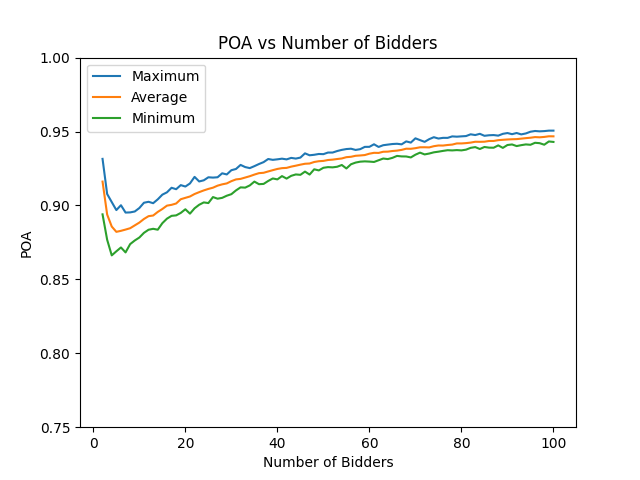
\includegraphics[scale=.8]{Figures/zi_symmetric}
	\caption{POA for 2 to 100 symmetric bidders}
	\label{zi_symmetric}
\end{figure}
 

 We see three things, one is that when all bidders are drawing from the same uniform distribution the market is incredibly efficient regardless of how smart the bidders are when choosing their strategy. Even with arbitrary strategies this auction still performs remarkably well. The second thing to note is that in this setting, as the number of bidders increases the social welfare also increases. This makes sense as we would expect the probability of a reasonably high valuation winning to increase as there are  more valuations per round. The third thing we notice, and most surprising of all, is that the increase in the price of anarchy as the number of players increases is not monotonic. At lower level of bidders, the efficiency actually decreases as we add more bidders. This seems to be because the probability that one player outbids another with a significantly higher valuation increases as you add players when you only have a few to begin with. Still though, the probability of someone with a high valuation winning is quite high and we see the price of anarchy approach 1 as $n$ goes to infinity. This is exactly what we expect as if we had a near infinite number of bidders, one of them would almost certainly bid arbitrarily close to their own valuation. 

We now conduct a similar simulation but with asymmetric bidders. In this case, half of the bidders are drawing uniformly from $[0,1]$ and half from $[0,2]$. The results are shown in table \ref{table:zero_int_asymmetric}. 

\begin{table}[h!]
	\begin{center}
		\begin{tabular}{ |c|c|c|c| }
			\hline
			Round & 2 Agent POA & 10 Agent POA & 100 Agent POA \\
			\hline
			1 & 0.1.000 & 1.0000 & 0.9726\\
			10 & 0.9115 & 0.8178 & 0.9331\\
			1,000 & 0.9054 & 0.8658 & 0.9310\\
			10,000 & 0.9092 & 0.8630 & 0.9297\\
			100,000 & 0.9112 & 0.8640 & 0.9304\\
			\hline
		\end{tabular}
		\caption{Price of anarchy in two player asymmetric auction}
		\label{table:zero_int_asymmetric}
	\end{center} 
\end{table}

Again we see that the market is quite efficient in this case regardless of how smart the bidders are. We again also see that it seems to converge to optimal (i.e. to 1) as the number of bidders increases but non-monotonically. We simulate this for 2 to 100 bidders again 10 times at each number of bidders with $T = 1,000$, where on odd numbers we allow the extra bidder to have distribution $[0,1]$. This is shown is figure \ref{figure:zi_assymetric}.

\begin{figure}[h!]
	\centering
	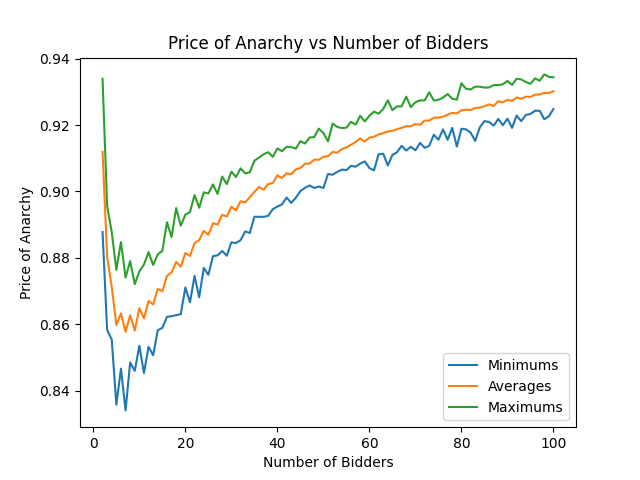
\includegraphics[scale=0.8]{Figures/zi_asymmetric}
	\caption{POA for 2 to 100 asymmetric bidders}
	\label{figure:zi_assymetric}
\end{figure}

Note that the baseline price of anarchy for minimal-intelligence agent auctions changes as we change the distributions. While the format seems quite efficient and well above the price of anarchy bounds (which again are only guaranteed for equilibria, which this is not) even with agents following these minimally intelligent strategies, we have no guarantee that there is not some way to construct this so that these agents wouldn't do much worse. Given that it seems as the number of agents increases, the efficiency also seems to increase, one would expect that this would need to be done by picking more interesting distributions for the bidders to choose from and only having two bidders.

\section{Simulating No-Regret Bidders}
With the results from the Bayes-Nash equilibrium demonstrated and an efficiency baseline established, we move on to simulating the bounds of no-regret learning agents in first-price auctions. Again, this is the equilibria we expect auctions to converge to if each agent is using a no-regret learning algorithm. To use these algorithms we do however have to make a concession to the environment we are simulating: we must now simulate an auction where the bidders are only allowed a finite number of actions.

\subsection{Multiplicative Weights Algorithm}
The no-regret learning algorithm we will use to train our bidders is called the multiplicative weights algorithm. It has been shown to satisfy the no-regret property in papers such as \citet{Littlestone1994} or \citet{Freund1999}, but our implementation of it comes from \cite{Roughgarden2016}. If each of our bidders use the no-regret learning algorithm our auction should converge to an outcome greater than the $0.63$ price of anarchy bound from chapter 2. 

Before giving the algorithm, a few words are probably necessary to understand where it comes from and what it is trying to do. First, this algorithm is what is called an {\em online} algorithm. That is an algorithm that takes its inputs sequentially as it goes rather than getting all of its inputs up front. Next, this algorithm and many other algorithms for players learning in games are based around the player only having a fixed number of actions they can choose from. For each round in the game, the player gets outside advice from "experts" who recommend to the player what to do at each round and the player picks among them to decide what to do. For us, these experts are our strategies that will map a valuation to a bid. At each time step $t$, the player picks the action to play and then after that, some adversary picks the utilities to assign for each action that could have been taken. This is a stronger condition than we will need as the adversary in a first-price auction is the cumulative action of the other players, where the highest bid determines which strategies (if any) the player could have taken and won. However, in the general case this algorithm has been shown to be no-regret in the face of an adversary directly picking the utilities the learning agent receives (see \cite{Lugosi2006} for a broad overview of prediction with expert advice and learning in games).\\

\begin{algorithm}[H]
	Initialize $w^1(a) = 1$ for every $a\in A$\\
	\For{$t = 1, 2, \ldots, T$}{
		Use distribution $p^t = \frac{w^t}{\sum_{a \in A} w^t(a)}$ over actions to pick $a \in A$ and output $a$.\\
		Given the utility vector $u^t$, for every action $a \in A$ use the formula $w^{t+1}(a) = w^t(a) \cdot (1 - \eta u^t(a))$ to update its weight.\\
		\caption{Multiplicative Weights (MW) Algorithm}
	}
\end{algorithm}
\vspace{1cm}
The logic of this algorithm is simple. At each time step we see how well each of the possible actions performed and increase the weight, or probability of selecting that action in the future. This increase is done proportionally to how well the action did as determined and \textit{learning rate}, $\eta$, is chosen before starting the procedure. As demonstrated in \cite{Roughgarden2016} and \cite{Blum2007}, the MW algorithm is no-regret if $\eta = \sqrt{(\ln n) / T}$ where $n$ is the number of actions that this agent can choose from, and $T$ is the number of rounds that will be played (yes, this assumes that the player knows that up front).

This algorithm fulfills our purpose of simulating agents learning in auctions, but in some sense it is unsatisfying that the learning algorithm requires a finite set of actions that the bidder does not even get to choose. It would be more interesting if we were able to give our agents some reasonable algorithm that allowed them to formulate their own strategies or mappings between their valuation and bid rather than choosing from a pre-made set. This would introduce a whole host of other problems from the reasonableness of expecting agents to implement such algorithms to the ability to prove that such algorithms converge to an equilibria. Part of the beauty of using multiplicative weights is that it is simple and has nice mathematical properties. Using more interesting learning techniques these properties might no longer hold and then we would have to wonder what our simulation is really showing\footnote{This thesis grew out of an interest in doing just that, throwing "smarter" algorithms such as neural networks and machine learning into existing multi-agent simulations. It becomes hard to tell what the point of such simulations are when the dynamics might just be properties of the interaction of the specific algorithms used and not of the system itself.}.

\subsection{Uniform Distribution Simulations}
The first simulation we run is a repeat of the symmetric auction setting, but now using agents learning with the multiplicative weights algorithm. We create 101 strategies that bidders can choose from to shade their bid, from bidding zero percent of their valuation with one percent increases up to bidding 100 percent of their valuation, $S = \{ 0, 0.01 \cdot v_i, 0.02 \cdot v_i, \ldots, 0.99 \cdot v_i, v_i \}$. First, we run the simulation with two symmetric bidders each choosing their valuation from the uniform distribution over $[0,1]$. The results are shown below in table \ref{table:3}.

\begin{table}[h!]
	\begin{center}
		\begin{tabular}{ |c|c| }
			\hline
			Round & POA \\
			\hline
			1 & 1.0000 \\
			10 & 0.9517 \\
			1,000 & 0.9129 \\
			10,000 & 0.9578 \\
			100,000 & 0.9947 \\
			\hline
		\end{tabular}
		\caption{Price of anarchy in two player asymmetric auction with no-regret learning}
		\label{table:3}
	\end{center} 
\end{table}

Here we can see that after 100,000 rounds the price of anarchy converges to 0.99 and near perfect efficiency as the agents learn how to play the game. It's important to point out here that the above table is not an average, but simply one run of the simulation. Since each time we run the simulation it is possible for the bidders to learn to converge to a new equilibrium, the POA values for each simulation can be different. While we are mainly concerned with the lowest possible POA that the system converges too as a demonstration of the proven bounds, it is also interesting to see what the average and best case simulations resulted in, as these will give us more confidence about the robust efficiency of the system. We now repeat this using 2 through 100 agents, each symmetric and drawing from a uniform $[0,1]$ as above. We run 100 simulations with each number of agents, each for 1,000 rounds\footnote{This is a relatively small number, but necessarily chosen for the sake of computation time with 100 agents who learn.}. This gives us the following results as shown in figure \ref{figure:symmetric} 

\begin{figure}[h!]
	\centering
	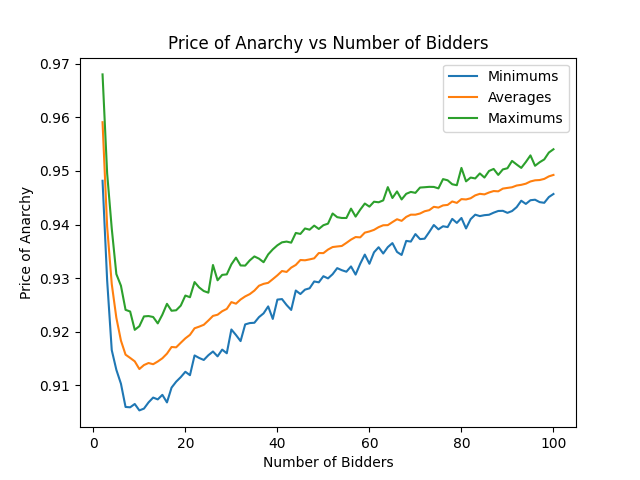
\includegraphics[scale=.8]{Figures/symmetric}
	\caption{POA for 2 to 100 symmetric, no-regret bidders}
	\label{figure:symmetric}
\end{figure}

The efficiency in the minimum case with our learning agents is about as good as the best-case with the random guessing agents. It makes sense that the efficiency would increase as we would expect people with higher valuations to win more often as people learn to minimize their regret. It is theoretically possible in some games that social welfare could be better off with everyone choosing arbitrary strategies than under learning agents, but we see in this game, and with our learning agents, that is not the case.  

Finally, we simulate the case of having two bidders with asymmetric valuation distributions where one draws uniformly from $[0,1]$ and the other draws from $[0,2]$. We can see the result of simulating this 100,000 times in table \ref{table:5} below.

\begin{table}[h!]
	\begin{center}
		\begin{tabular}{ |c|c| }
			\hline
			Round & POA \\
			\hline
			1 & 1.0000 \\
			10 & 0.8901 \\
			1,000 & 0.9314 \\
			10,000 & 0.9770 \\
			100,000 & 0.9961 \\
			\hline
		\end{tabular}
		\caption{Price of anarchy in two player asymmetric auction with no-regret learning}
		\label{table:5}
	\end{center} 
\end{table}

Here we see the agents converge to a very good efficiency similar to the behavior we saw when using the Bayes-Nash equilibrium for this setting and better than in the two bidder minimum-intelligence case. Now again we conduct this simulation with 2 to 100 asymmetric bidders. For each number of bidders we simulate this 100 times and when there are an odd number of bidders there is an extra $[0,1]$ bidder. Each sequential auction consists of 100,000 rounds. The results are shown in figure \ref{figure:asymmetric}.

\begin{figure}[h!]
	\centering
	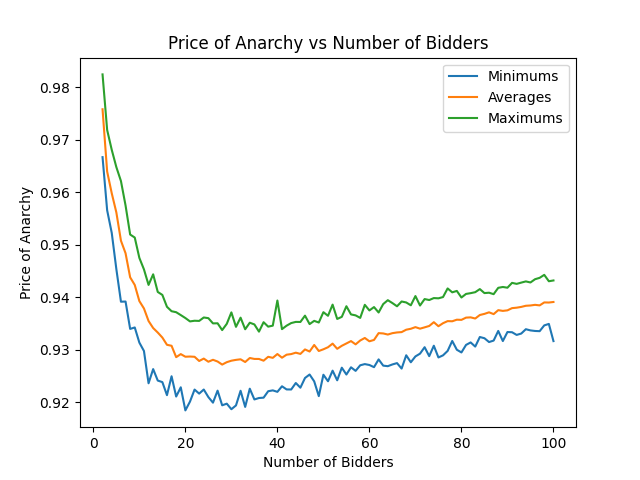
\includegraphics[scale=.8]{Figures/asymmetric}
	\caption{POA for 2 to 100 asymmetric, no-regret bidders}
	\label{figure:asymmetric}
\end{figure}

Figure \ref{figure:asymmetric} is similar to the figures we  have seen for every other auction. We see very high efficiency for two or three bidders, and then see a dramatic decrease as it goes to 9. We then see the numbers slowly climb back towards being fully efficient in the best, worst, and average cases. Comparing the results of our simulations, we see that while the asymmetric learners were more efficient for lower levels of bidders, they do not approach fully efficient in the same way symmetric no-regret bidders do as $n$ grows. Rather, it starts to level off faster. This seems reasonable based off of our expectations and similar results with minimally intelligent bidders.

\chapter*{Conclusion}
         \addcontentsline{toc}{chapter}{Conclusion}
	\chaptermark{Conclusion}
	\markboth{Conclusion}{Conclusion}
	\setcounter{chapter}{4}
	\setcounter{section}{0}
	
Our simulation demonstrated the efficiency greater than the price of anarchy bounds with no-regret bidders. The price of anarchy theorems that give the bounds for the efficiency of the system tell us that these should hold no matter what number of bidders and what distributions we give them. By all indications with both learning, and non-learning agents first-price single-item auctions are incredibly efficient. It makes one wonder how low one could get the simulated price of anarchy to be. It also begs for a better proof giving the exact lower bound on the price of anarchy for no-regret learners. Combining the results from the learning and non-learning agents we should feel incredibly confident in the efficiency of first-price auctions implemented in the real world. It seems like they behave remarkably well as a way to allocate resources to those who value them the most. 

Moving forward using simulations to understand the price of anarchy in auctions, there are two obvious ways to extend this research. One is to build a simulation for simultaneous first-price auctions or all-pay auctions (where everyone must pay regardless of winning) where the price of anarchy bounds for no-regret agents have also been proven using smooth-auctions (Definition \ref{dfn:smoothauction}) \citep{Roughgarden2017}. For simultaneous auctions, or any sort of auction where bidders must make many decisions at once (in this case bids), simulating no-regret learning becomes much harder as the number of actions increases. The simulations presented here were already slow, its hard to imagine how long it would take to run a simulation of such a procedure. The other obvious extension is to try simulating this again using different algorithms. Specifically we could try different no-regret algorithms and see if they converge to similar efficiency outcomes, but it might also be interesting to try modern machine learning techniques. Again, if one uses techniques that don't allow us to bound the efficiency of their outcomes, it can be hard to know how sensitive the results are to particular parameters or what it might possibly do in every scenario. That is why no-regret learning is so nice as a stand in for humans. It is simple to implement, it is well behaved, and it is boundable. Hence, we should also expect human agents learning in auctions to make choices that lead to mostly efficient outcomes.


%If you feel it necessary to include an appendix, it goes here.
    \appendix
      \chapter{Simulation Code}
      The code for this simulation is available at the public GitHub repository:
      \begin{center}
      	\url{https://github.com/15rsirvin/Computational-Economics}
      \end{center}
      in the sequential auction folder. 
      There are different Python files for each of the simulations where the relevant parts are changed to make them minimally intelligent bidders or asymmetric. The simulation is coded in Python and mostly consists of loops to sequentially run each auction, update each bidder, and then allow each bidder to learn. We run each simulation in parallel on a different processor to try and speed up the process, but is is still quite slow for large numbers of simulations, rounds, or bidders. That is because this process is essentially $O(T \cdot n \cdot m)$, where $T$ is the number of rounds, $n$ the number of bidders, and $m$ is the number of simulations at that number of bidders. 
      
      We ran our code on a google cloud platform "compute engine" server to speed up the simulation process with a faster computer and to allow the simulation to run continuously. This enabled us to choose high values of $T, m,$ and $n$, despite how long the code takes to execute with such values.  
      
      If someone were to try and replicate parts of this thesis, I would recommend re-writing the code in a faster language like C or C++. Because this code scales linearly with any individual input, optimizing the speed at which the loop executes should have a massive effect on the total time it takes to compute. It might also be possible to algorithmically optimize this simulation so that it can scale sub-linearly. Ultimately we decided not to spend to much time optimizing the code as letting it run on a remote server was not a huge issue.
      

%This is where endnotes are supposed to go, if you have them.
%I have no idea how endnotes work with LaTeX.

  \backmatter % backmatter makes the index and bibliography appear properly in the t.o.c...

% if you're using bibtex, the next line forces every entry in the bibtex file to be included
% in your bibliography, regardless of whether or not you've cited it in the thesis.
    \nocite{*}

% Rename my bibliography to be called "Works Cited" and not "References" or ``Bibliography''
% \renewcommand{\bibname}{Works Cited}

%    \bibliographystyle{bsts/mla-good} % there are a variety of styles available; 
%  \bibliographystyle{plainnat}
% replace ``plainnat'' with the style of choice. You can refer to files in the bsts or APA 
% subfolder, e.g. 
 \bibliographystyle{APA/reedecon}  % or
 \bibliography{thesis}
 % Comment the above two lines and uncomment the next line to use biblatex-chicago.
 %\printbibliography[heading=bibintoc]

% Finally, an index would go here... but it is also optional.
\end{document}
